%% 
%% Copyright 2007-2019 Elsevier Ltd
%% 
%% This file is part of the 'Elsarticle Bundle'.
%% ---------------------------------------------
%% 
%% It may be distributed under the conditions of the LaTeX Project Public
%% License, either version 1.2 of this license or (at your option) any
%% later version.  The latest version of this license is in
%%    http://www.latex-project.org/lppl.txt
%% and version 1.2 or later is part of all distributions of LaTeX
%% version 1999/12/01 or later.
%% 
%% The list of all files belonging to the 'Elsarticle Bundle' is
%% given in the file `manifest.txt'.
%% 
%% Template article for Elsevier's document class `elsarticle'
%% with harvard style bibliographic references

%\documentclass[preprint,12pt,authoryear]{elsarticle}

%% Use the option review to obtain double line spacing
\documentclass[authoryear,preprint,review,12pt]{elsarticle}

%% Use the options 1p,twocolumn; 3p; 3p,twocolumn; 5p; or 5p,twocolumn
%% for a journal layout:
%% \documentclass[final,1p,times,authoryear]{elsarticle}
%% \documentclass[final,1p,times,twocolumn,authoryear]{elsarticle}
%% \documentclass[final,3p,times,authoryear]{elsarticle}
%% \documentclass[final,3p,times,twocolumn,authoryear]{elsarticle}
%% \documentclass[final,5p,times,authoryear]{elsarticle}
%% \documentclass[final,5p,times,twocolumn,authoryear]{elsarticle}

%% For including figures, graphicx.sty has been loaded in
%% elsarticle.cls. If you prefer to use the old commands
%% please give \usepackage{epsfig}

%% The amssymb package provides various useful mathematical symbols
\usepackage{amssymb}
%% The amsthm package provides extended theorem environments
%% \usepackage{amsthm}

\usepackage{siunitx}  % for degree celsius
\usepackage{multirow} % for the table
\usepackage{booktabs} % fot toprule, midrule
\usepackage{longtable}

\usepackage{color,soul} % highlight 

% for track changes in revision version, comment this one if want the final version
\usepackage{changes}
%\usepackage[final]{changes}

\usepackage{hyperref} %for breaking long url

%% The lineno packages adds line numbers. Start line numbering with
%% \begin{linenumbers}, end it with \end{linenumbers}. Or switch it on
%% for the whole article with \linenumbers.
%% \usepackage{lineno}

\usepackage{lineno}
\linenumbers

\journal{Remote Sensing of Environment}

\begin{document}

\begin{frontmatter}

%% Title, authors and addresses

%% use the tnoteref command within \title for footnotes;
%% use the tnotetext command for theassociated footnote;
%% use the fnref command within \author or \address for footnotes;
%% use the fntext command for theassociated footnote;
%% use the corref command within \author for corresponding author footnotes;
%% use the cortext command for theassociated footnote;
%% use the ead command for the email address,
%% and the form \ead[url] for the home page:
%% \title{Title\tnoteref{label1}}
%% \tnotetext[label1]{}
%% \author{Name\corref{cor1}\fnref{label2}}
%% \ead{email address}
%% \ead[url]{home page}
%% \fntext[label2]{}
%% \cortext[cor1]{}
%% \address{Address\fnref{label3}}
%% \fntext[label3]{}

%\ead{huanglingcao@link.cuhk.edu.hk}

\title{Using Deep Learning to Map Retrogressive Thaw Slumps in the Beiluhe Region (Tibetan Plateau) from CubeSat Images}

%\title{Mapping Retrogressive Thaw Slumps in the Beiluhe Region (Tibetan Plateau) from CubeSat Images using Deep Learning}

%% use optional labels to link authors explicitly to addresses:
%% \author[label1,label2]{}
%% \address[label1]{}
%% \address[label2]{}

\author[a]{Lingcao Huang}
\author[b]{Jing Luo}
\author[b]{Zhanju Lin}
\author[b]{Fujun Niu}
\author[a]{Lin Liu}


\address[a]{Earth System Science Programme, Faculty of Science, The Chinese University of Hong Kong, Hong Kong SAR, China.}
\address[b]{Northwest Institute of Eco-Environment and Resources, Chinese Academy of Sciences, Lanzhou, China.}

\begin{abstract}

Retrogressive thaw slumps (RTS\added{s}) are among the most dynamic landforms in permafrost areas, and their formation can be attributed to the thawing of ice-rich permafrost. The spatial distribution and impacts of RTSs on the Tibetan Plateau are poorly understood \replaced{due to}{, because of} their remote location and the technical challenges of automatic mapping. In this study, we innovatively applied DeepLabv3+, a cutting-edge deep learning algorithm \added{for semantic segmentation}, to Planet CubeSat images, which are satellite images with high spatial and temporal resolution. Our method allows us to automatically delineate \replaced{220}{196} RTSs within an area of \replaced{5200}{7500} km$^2$ with an average precision of \replaced{0.541}{0.536}. The corresponding precision, recall, and F1 score are \replaced{0.863, 0.833, and 0.848}{0.842, 0.817, and 0.829,} respectively \replaced{when the threshold of intersection over union is 0.5.}{(under the IOU threshold of 0.5).} \added{Moreover, approximately 100 experiments show that our method is robust.} We find that (1) most of the RTSs are small (areas $<$ eight ha and perimeters $<$ 2000 m) and (2) RTSs preferentially develop at locations with gentle slopes (four to eight degrees), and in areas lower than the surroundings (the mean \replaced{topographic position index}{TPI} is $-0.17$) and \replaced{receiving}{which receive} less solar \replaced{radiation}{radiations} (i.e., north-facing slopes). The results show that the method can map RTSs automatically from Planet CubeSat images and can potentially be applied to larger areas.


\end{abstract}

\begin{keyword}
%% keywords here, in the form: keyword \sep keyword

%% PACS codes here, in the form: \PACS code \sep code

%% MSC codes here, in the form: \MSC code \sep code
%% or \MSC[2008] code \sep code (2000 is the default)
Convolutional neural network \sep Planet CubeSat  \sep Permafrost Thawing  \sep Retrogressive Thaw Slumps \sep Tibetan Plateau.

\end{keyword}

\end{frontmatter}

%% \linenumbers
%\tableofcontents

%% main text
\section{Introduction}
\label{sec_intro}

Permafrost underlies approximately 24\% of the exposed land surface in the northern hemisphere \citep{zhang_statistics_1999} and undergoes warming as well as degradation. Borehole measurements have shown that the permafrost is undergoing \deleted{strong} warming  \citep{marchenko_permafrost_2007,osterkamp2005recent,romanovsky_thermal_2010,romanovsky_permafrost_2010,wu2008Recent,zhao_thermal_2010,biskaborn2019permafrost}. The warming of permafrost can cause \added{degradation through active layer thickening and development of thermokarst landforms} \deleted{ its degradation such as active layer thickening, shrinking in its area, and development of thermokarst landforms} \citep{zhao_thermal_2010,aakerman2008thawing,czudek_thermokarst_1970,jorgenson_response_2005,osterkamp_characteristics_2007}. Furthermore, permafrost degradation can cause damage to infrastructure, release greenhouse gases from decayed carbon stored in permafrost, and significantly alter the local ecosystem \citep{tong_effect_1996,grosse_vulnerability_2011,olefeldt_circumpolar_2016,schuur_climate_2015,schuster2018permafrost}. On the Tibetan Plateau, permafrost underlies a total area of about 1.06$\times10^6$ km$^2$ and is shallow (thinner than 100 m) as well as warm (higher than \SI{-2}{\celsius}) \citep{zhou_geocryology_2000}. Therefore, permafrost on the Tibetan Plateau is sensitive and vulnerable to climate changes and anthropogenic disturbance. %Mapping and monitoring the changes in permafrost areas are essential to understanding the impacts and consequences of permafrost degradation. 

A retrogressive thaw slump (RTS) is one of \replaced{many kinds}{over 20 types} of thermokarst landforms resulting from the thawing of ice-rich permafrost \added{\citep{czudek_thermokarst_1970, jorgenson_response_2005, jorgenson_thermokarst_2013,kokelj2013advances,farquharson2016spatial,jones2019rapid}} \deleted{(Czudek and Demek, 1970; Jorgenson and Osterkamp, 2005; Jorgenson, 2013; Kokelj and Jorgenson, 2013)}. Several triggering mechanisms including lateral stream erosion and active layer detachments are responsible for RTSs \citep{french2017periglacial}. Commonly, a detachment slide removes the soil above permafrost and exposes it to rapid thawing, then initiates an RTS. Retrogressive thawing of permafrost at the exposed headwall further expands the thawed area towards the upslope \deleted{(Jorgenson, 2013). T}\added{,t}ypically, the maximum retreat rates are 6--8 meters per year \citep{jorgenson_thermokarst_2013}. Once an RTS initializes, it can be active for decades \citep{burn1989geomorphology, lacelle2010climatic, swanson2018growth,lewkowicz2019extremes} and has significant impacts on the local and downslope ecosystem \added{such as mass wasting of soil as well as vegetation \citep{gooseff2009effects} and increases of mercury concentrations \citep{pierre2018unprecedented}}. \deleted{(Gooseff et al., 2009; Pierre et al., 2018; Zolkos et al., 2018)}

RTSs can occur throughout permafrost areas, but many of them \replaced{remain}{are} unmapped, especially those on the Tibetan Plateau. Many studies have investigated RTSs in northern and central Alaska (e.g., \citealp{swanson2018growth,balser2014timing}), northern Canada (e.g., \citealp{burn1990canadian, cassidy2017impacts, armstrong2018thaw,lewkowicz2019extremes}), and Siberia (e.g., \citealp{leibman2003dynamics, zwieback2018sub}). % and the Tibetan Plateau (e.g., \citealp{niu2005engineering, niu2016thaw}). 
Compared with these Arctic and subarctic regions, however, the RTSs on the Tibetan Plateau have received much less investigation. 
A few studies focused on one or several RTSs near the Qinghai-Tibet Highway (e.g., \citealp{wang1995situ,sun2017creep}). The only regional studies to date have targeted an area along the Qinghai-Tibet Engineering Highway \added{\citep{niu2014thaw, niu2016thaw,luo2019recent}}\deleted{(Niu et al., 2014, 2016)}. 
%Due to the limitations of mapping methods, these are site-focused or regional studies. 
The distribution and impacts of RTSs in large permafrost areas on the Tibetan Plateau are poorly quantified and understood. 
Possible reasons include (1) most of them are in remote and inaccessible regions and (2) they are similar to the surroundings or other landforms, which makes it challenging to map them from remote sensing images.

\replaced{Images taken by}{The images from} CubeSats enable us to map the spatial distribution of RTSs on the Tibetan Plateau. CubeSats, small and low-cost satellites, can provide high spatial and temporal resolution images by deploying them in a multi-satellite constellation. \added{Since 2013,} Planet (also known as Planet Labs; \url{planet.com}) has deployed \added{around 300 CubeSats. After 2017,} more than 150 \replaced{of them}{CubeSats} are active in sun-synchronous orbits and \replaced{collect}{collects} daily images \added{with four bands} of the global land surface at 3--5 m resolution. These images have great potential for earth observation and have been used in many studies, such as water body tracking \citep{cooley2017tracking, cooley2019arctic, aragon2018cubesats, miles2018glacial}, vegetation \citep{houborg2016high, houborg2018daily}, and glacier investigation \citep{altena2017glacier}. In this study, we collect images \replaced{over}{of} our study area from the PlanetScope constellation (hereafter referred to as “Planet images”), which have a spatial resolution of 3 m and are sufficient for delineating most RTSs. The high temporal resolution of Planet images enables cloudless images to be acquired which cover the whole study area within one month, even \added{in} areas with frequent cloud cover. With the high spatial resolution, we can map many small RTSs, including one with an area smaller than a hectare previously reported \added{by} \cite{niu2012development,niu2016thaw}, and accurately delineate their boundaries. These small RTSs do not show up well on Landsat images because of its coarse resolution (30 m) although these images \replaced{have been}{were} used to map RTSs \added{with large surface areas} in circumpolar areas \citep{lacelle_distribution_2015, brooker2014mapping, nitze2018remote}. %The accurate boundaries of RTSs are essential for quantifying their temporal changes. 

To automatically map RTSs, which is necessary for a large area, we \replaced{applied innovative}{ innovatively apply} deep learning algorithms to Planet images. Previous studies (e.g., \citealp{ramage_terrain_2017, lantuit_fifty_2008, niu2014thaw}) combined field investigation and manual delineation on high-resolution remote sensing images to obtain RTS inventories, which are time-consuming and limited to small areas. Compared with thermokarst lakes, RTSs are complex landforms and are difficult to automatically map on images. An RTS consists of headwall, slump floor, slump lobe, and head scarp \citep{lantuit_fifty_2008}. Different parts of RTSs have different colors on images because of various soil types, water content, incoming solar angles, and vegetation. In some regions with sparse vegetation, the colors of RTSs are quite similar to other land covers such as bare lands. Therefore, the diverse radiometric characteristics and the similarity to their surroundings require a mapping method which has a high capability that can represent their obscure features. Deep learning \deleted{algorithms} \added{outperformed other algorithms in image classification with a large margin \citep{krizhevsky_imagenet_2012} and has dramatically improved image processing technology \citep{lecun_deep_2015}}. \deleted{have been used in many complex scenarios and achieved unprecedented results \text{(e.g., \citealp{krizhevsky_imagenet_2012, lecun_deep_2015, silver_mastering_2017})}} In remote sensing applications, deep learning has also achieved outstanding results in land cover mapping, object detection, \deleted{poverty estimation,}and delineation of ice-wedge polygons \replaced{\textnormal{\citep{guo_geospatial_2018, zhang2018deep,abolt2019brief}}}{\text{\citep{jean_combining_2016, guo_geospatial_2018, zhang2018deep}}}. However, none of these studies have targeted RTSs. 

The objectives of this study are: (1) to automatically map RTSs \replaced{using}{on} Planet images, based on deep convolutional neural networks and (2) to analyze the relation between the spatial distribution and terrain factors in the Beiluhe region on the Tibetan Plateau. We applied DeepLabv3+, one of the best semantic segmentation algorithms, to Planet images and conducted numerous experiments using different settings. By comparing with manual delineations, we calculated the accuracies of mapped results and assessed the performance of our method. We quantified their geometric characteristics of the mapped RTSs and analyzed the relationship between their spatial distribution and terrain factors. We also discuss the advantages and limitations of using Planet images as well as the automatic mapping method. 
To the best of our knowledge, this is the first study on mapping landforms related to the thawing of ice-rich permafrost using CubeSat images, and will provide an assessment of deep learning applications on the Tibetan Plateau.
%The numerous experiments will provide an assessment of the application of deep learning algorithms for mapping targets on Tibetan Plateau using images with a similar resolution. 


\section{Study area}
\label{sec_studyarea}
The study area ($92.50^\circ$E to $93.51^\circ$E, $34.69^\circ$N to $35.18^\circ$N) is in the Beiluhe region on the Tibetan Plateau (Fig. \ref{fig_rts_groundphoto}\added{a}), with an approximate size of \replaced{5200}{7500} km$^2$. The elevation ranges from 4418 m to 5320 m, with a mean of 4673 m. The records from a nearby meteorological station ($93.08^\circ$E, $35.22^\circ$N) show that the mean annual air temperature and annual precipitation are \SI{-3.8}{\celsius}, and around 300 mm, respectively \citep{luo_thermokarst_2015}. The vegetation includes alpine meadow (occupies \textgreater 45\% of the area) and alpine grassland (occupies \textless 20\% of the area) \citep{luo_thermokarst_2015}. 

Most of this area is underlain by ice-rich permafrost: 70\% of the area \replaced{has}{with} a volumetric ice content higher than 30\%, 
%, while 20\% has ice contents \textgreater 50\%, 
and the thickness of permafrost ranges from 20 to 80 m \citep{zhou_geocryology_2000, luo_thermokarst_2015}. \added{According to the in situ observations from over 40 boreholes in the study area, the type of ground ice is mainly massive ice, whose formation is due to repeated-segregation \citep{guodong1983mechanism}.} The mean annual ground temperature \added{at ($\sim$15 m) the depth of zero annual amplitude}\deleted{ of the entire area} is between \SI{-2.0} and \SI{-0.5}{\celsius}, and the active layer thickness is between 1.5 and 2.0 m \citep{zhou_geocryology_2000, luo_thermokarst_2015, wu2010changes, wu2015changes}. % \hl{ More information? (air/ground temperature change?)}  %TODO:  need co-authors to add more information on study area, from Luo jing's reply, there is no more data.

\begin{figure}
	\centering
	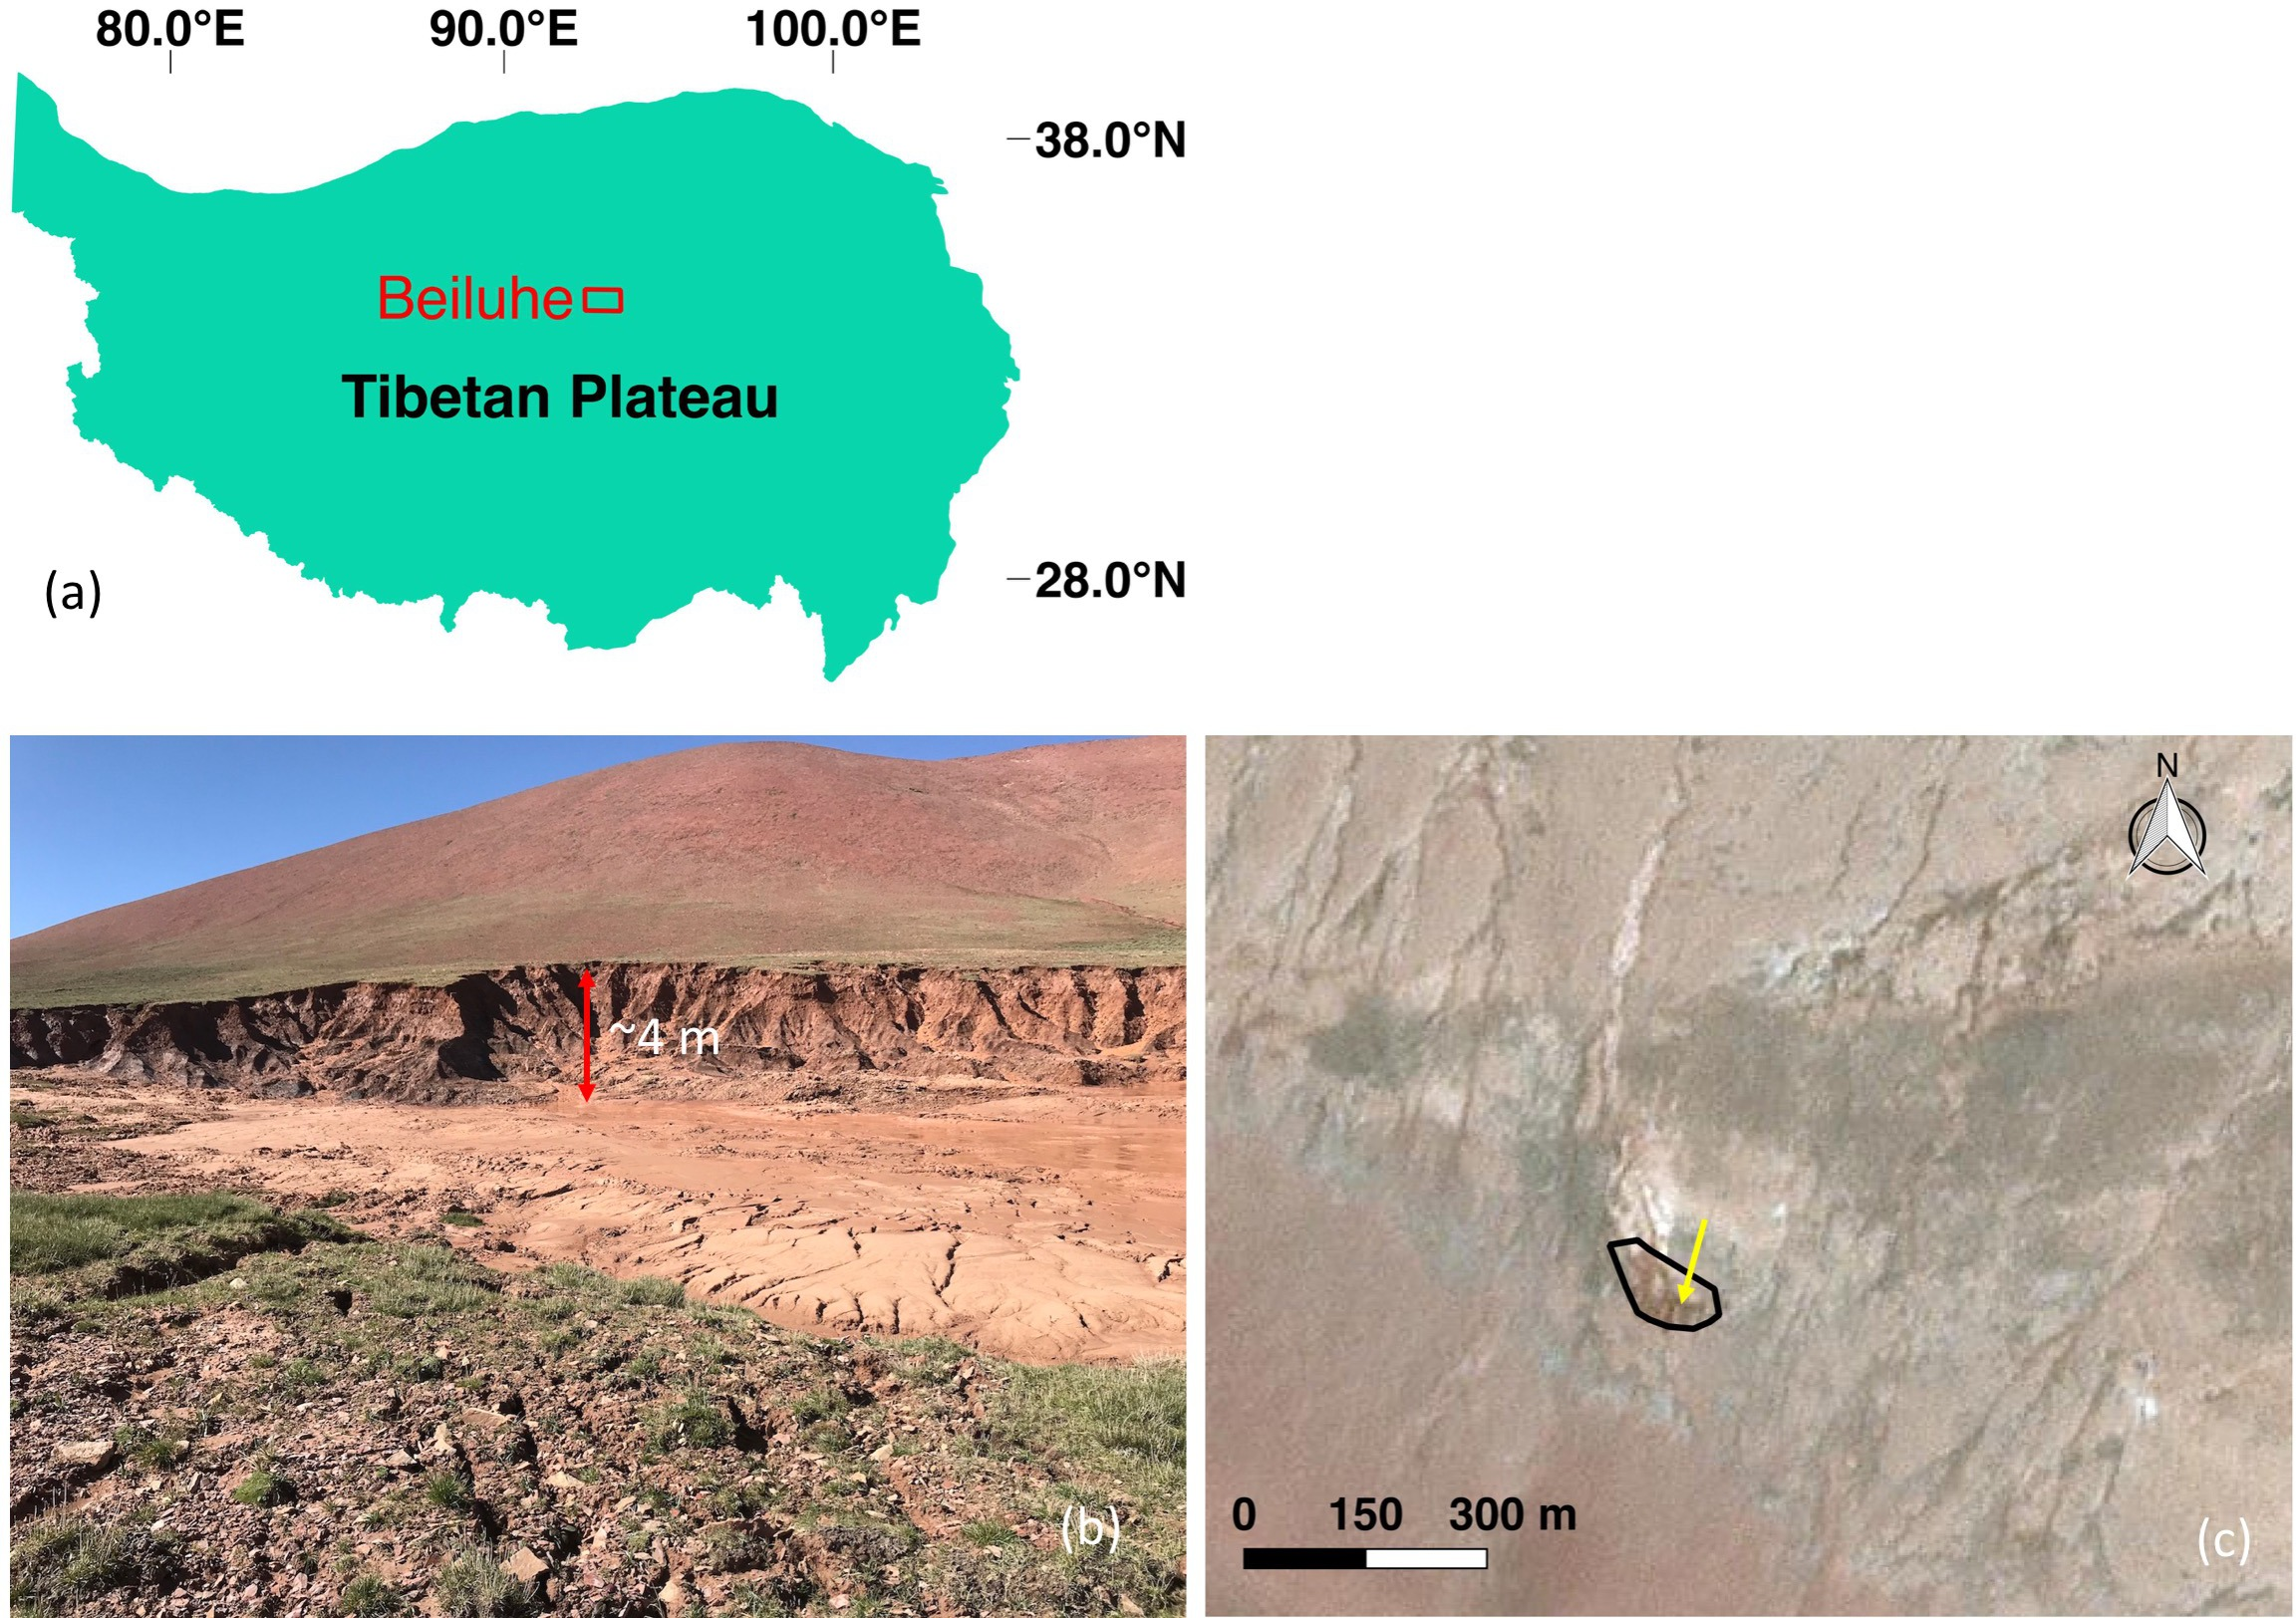
\includegraphics[width=14cm]{figures/study_area_loc_RTS_photo_v2_trim.jpg}
	\caption{\added{The study area and a retrogressive thaw slump (RTS). The red rectangle in (a) shows the extent of our study area on the Tibetan Plateau. (b) and (c) are the ground photo and Planet image of an RTS whose central location is 92.912 $^\circ$E, 34.848 $^\circ$N. In (c), the black polygon outlines the RTS; the yellow arrow indicates the facing direction of the ground photo}. \deleted{The ground photo (a) and Planet image (b) of a retrogressive thaw slump (RTS) whose central location is 92.912 $^\circ$E, 34.848 $^\circ$N. In (b), the black polygon outlines the RTS, the yellow arrow indicates the facing direction of the ground photo, and the inset shows the location of our study area on the Tibetan Plateau.}}
	\label{fig_rts_groundphoto}
\end{figure}

RTSs are one of the typical \replaced{thaw-related}{ thermokarst} landforms in this area. Fig. \ref{fig_rts_groundphoto}\replaced{b}{a} shows the ground photo of an RTS. Its size is about 0.9 ha and the headwall height is around four meters. Fig. \ref{fig_rts_groundphoto}\replaced{c}{b} shows the corresponding Planet images with red, green, and blue bands. 

\section{Methods}
\label{sec_meth}

\subsection{Collection and Pre-processing of Planet images}
\label{subsec_collect_images}

We downloaded Planet images via the Planet website (\url{www.planet.com}) through its Education and Research Program. We downloaded 64 PlanetScope scenes of images (\replaced{termed as}{as known as} Daily Imagery \added{by Planet}). Each scene covers an area of around 10 km by 30 km and has four bands (blue, green, red, and near-infrared). The acquisition dates were 22 and 23 May 2018. The product level we chose was ``Analytic'', which means that the images had been orthorectified, and \replaced{their pixel values represent}{ converted to} surface reflectance. Moreover, the bit depth and positional accuracy are 16 bit and higher than 10 m, respectively. %Planet also provides mosaic images but only available for commercial request. 

We pre-processed the Planet images according to the requirement of the deep learning algorithm and manual delineation. For the 64 scenes, we mosaicked and extracted red, blue, and green (RGB) bands using Geospatial Data Abstraction Library (GDAL, \url{gdal.org}), then stretched and sharpened the images using OpenCV (\url{opencv.org}). Since the deep learning algorithm (DeepLabv3+) used in this study only accepts three image bands as input, we conducted experiments to decide the best approach to extract three bands from Planet images. The candidate approaches include (1) extracting RGB bands since they are a natural color and will facilitate manual identification, (2) combining \deleted{of} normalized difference vegetation index (NDVI) \citep{rouse1974monitoring}, normalized difference water index (NDWI) \citep{mcfeeters1996use}, and the blue band (excluded when calculating NDVI and NDWI), and (3) adopting the first three \replaced{bands}{ components} after \added{applying} principal component analysis (PCA) \added{to the 4-band Planet images}. Because RTS formation results in an abrupt change of land cover in vegetation and soil moisture, \replaced{including}{ the combination of} NDVI and NDWI can help identify RTSs on images. PCA \replaced{uses an orthogonal transformation to re-organize a set of values}{ is a statistical procedure that re-organizes the information} in descending order \added{of their variance} \citep{wold1987principal}. \added{We used ``Orfeo Tool Box'' \citep{inglada2009orfeo} to conduct PCA transformation then only kept the first three components as the bands of the new images.} By using PCA, we can keep the maximum amount of information on Planet images when \replaced{reducing 4-band images}{converting the original images} to \replaced{3-band ones}{three bands}. 
%We adopted the approach of extracting RGB bands for pre-processing because it achieved the highest accuracy (see section \ref{subsec_otherbands}).
 After pre-processing, we obtained a mosaic image (30916 pixels by 18713 pixels) as the input to the automatic mapping method and manual delineation. \replaced{Unless stated otherwise}{ If not explicitly stated,} the Planet image refers to this mosaic one in the remainder of this paper.

\subsection{Collection of Ground Truth Polygons}
\label{subsec_collect_groundtruth}

We manually delineated RTSs \added{throughout the entire study area} on Planet images in QGIS (version 2.18.14, \url{qgis.org}) and conducted fieldwork to validate them. We divided the total study area into 1410 square grids using the vector-grid tool in QGIS. The size of each grid was 2.3 km$\times$2.3 km. RTSs in each grid were independently delineated by two researchers with extensive experience of mapping RTSs. 
%Inconsistent result were decided with the third researcher. 
The criteria for mapping RTSs were based on their distinct morphologic and tonal characteristics, including the presence of a headwall, slump floor or toe, the absence of vegetation, and the \replaced{polycyclic}{RTS} shape. We cross-checked \replaced{70}{90}\% of the manual results by visiting them in the field in 2014 and 2018 and all of them by visual checking \added{on images} from Google Earth \added{and other satellites including WorldView-1, SPOT-5, and Gaofen-1 \citep{luo2019recent}}. Around \replaced{30}{10}\% of \replaced{them}{the RTSs} were difficult to reach in the field. In total, we obtained \replaced{263}{202} polygons of RTSs as ground truths.  

\subsection{Automatic mapping of RTSs}
\label{subsec_auto_mapping}

Fig. \ref{fig_flowchart} shows the flowchart of our automatic mapping method. Firstly, we converted boundaries of landforms (i.e., ground truths) and a portion of Planet images to training and label images. Secondly, we trained the neural network and obtained its parameters. Next, we inputted the Planet image of the entire study area and predicted RTSs. After post-processing, we obtained mapped polygons of RTSs. Lastly, we validated the mapped polygons and calculated their accuracy. The details of each step are described below.

\begin{figure}[ht]
	\centering
	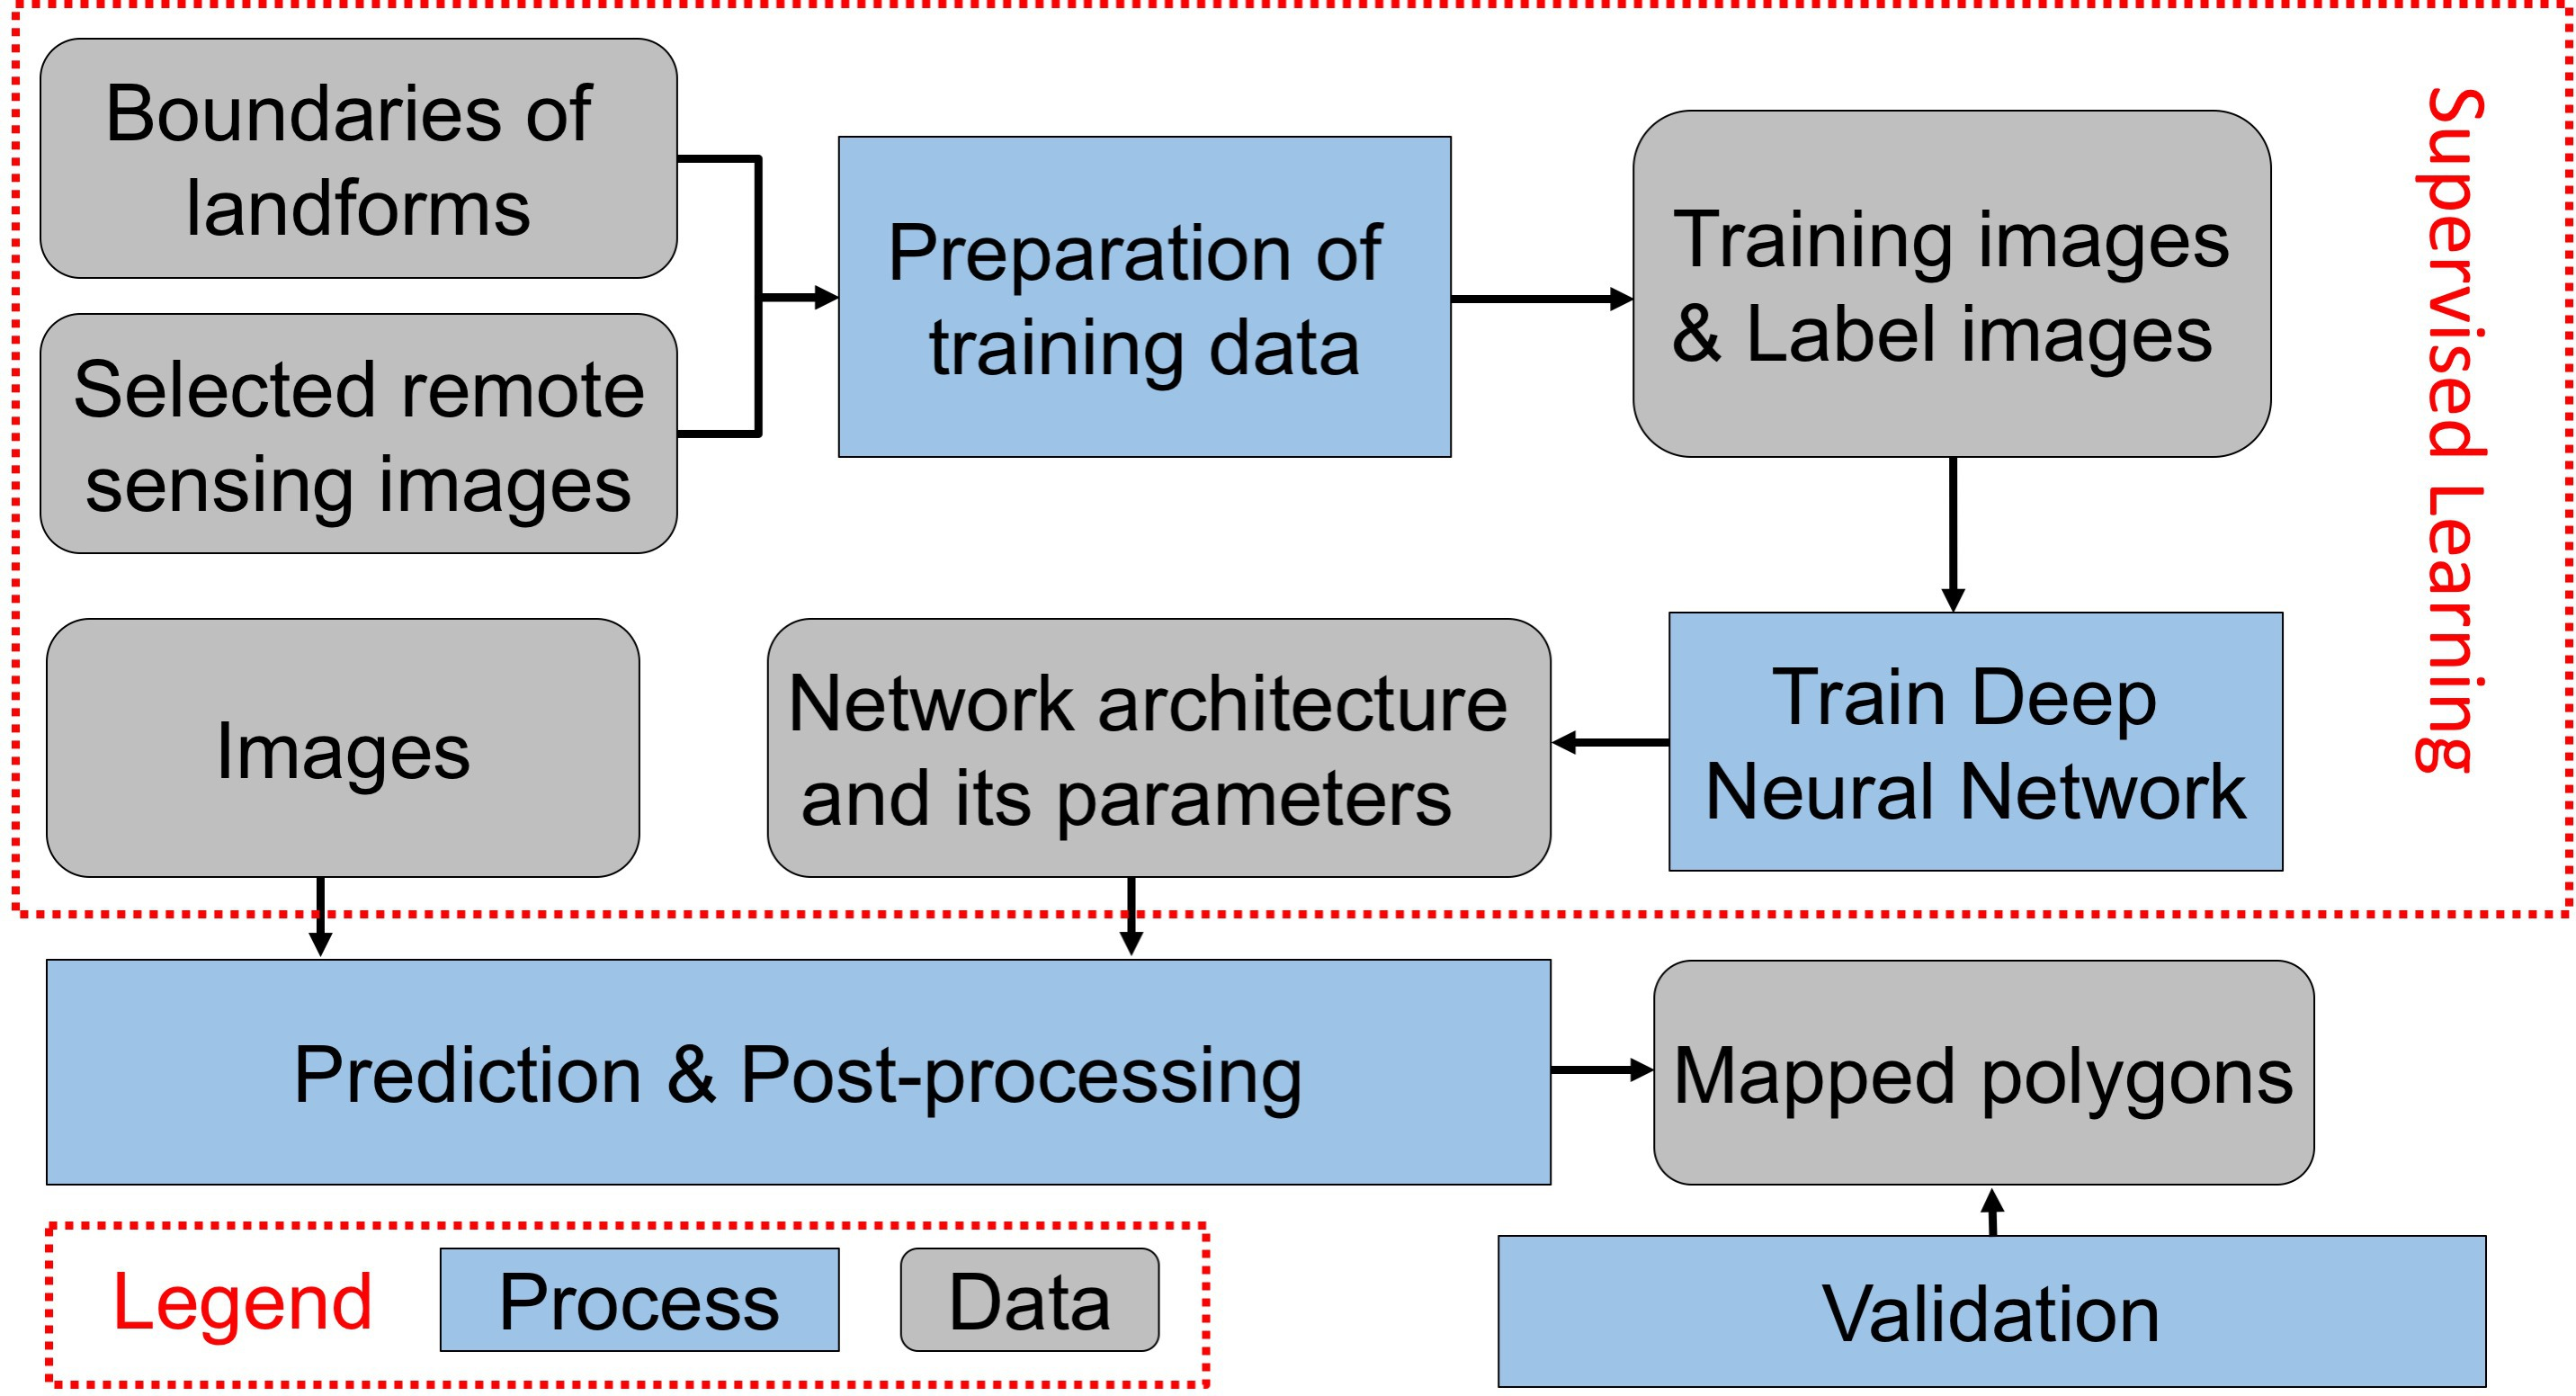
\includegraphics[width=12cm]{figures/flowchart_trim.jpg}
	\caption{Flowchart of the automatic mapping method based on deep learning algorithms.}
	\label{fig_flowchart}
\end{figure}

\subsubsection{Preparation of training data}
\label{subsubsec_pre_trainingdata}

We derived training data by choosing all the ground truths as positive training polygons and \replaced{94}{104} non-RTS polygons as negative ones. The non-RTS polygons cover other land covers such as vegetation, bare land, and water bodies. To make the non-RTS polygons representative for training, we ran an initial mapping exercise \replaced{by only using ground truths as training polygons}{excluding negative samples}, then we \replaced{added}{delineated} non-RTS polygons to cover areas containing numerous false positives (defined in section \ref{subsubsec_validation}). \replaced{This method}{It} is practical to choose negative samples that are similar to RTSs. Otherwise, creating non-RTS polygons requires expertise and ground knowledge of all the land covers in the study area. Since the surrounding area of an RTS contains context information, we set a buffer area of 300 meters and then extracted a subset of Planet images (hereafter referred to as “sub-image”). Fig. S1, S2, and S3 in the Supplementary Materials show the distribution and extent of the training polygons and sub-images. The sub-images only covered \replaced{6.91}{6.03}\% (\replaced{2.06}{1.35}\% and \replaced{4.85}{4.68}\% derived from positive and negative training polygons, respectively) of the entire study area. Furthermore, we subdivided a sub-image into patches by setting a patch size as 480 pixels with an overlap of 160 pixels. \added{The overlap is critical to identify all pixels of one RTS that appears in two or more patches.} We rasterized ground truth polygons then derived label images from the raster. The technical details of obtaining training images and label images are described in greater detail \added{by \cite{huang2018automatic}.} \deleted{in a previous study \text{\citep{huang2018automatic}}.} 

To improve the quantity of training data and generalization of the mapping method, we applied data augmentation to the positive patches. \added{Data augmentation is an approach to increase the quantity as well as the diversity of training data and is necessary for this study because it can enrich our limited training data.} We excluded the negative patches during data augmentation because their quantities are sufficient for training. The most common data augmentation practices include flipping, blurring, cropping, scaling, and rotating. In this study, we utilized the implementation of these methods in a \replaced{Python package named ``imgaug"}{“imgaug” package} (\url{imgaug.readthedocs.io}). Specifically, we adopted flipping (left and right as well as up and down), blurring (gaussian blur with sigma equal to one and two), cropping (10 and 30 pixels), scaling (with factors are 0.75 and 1.25), and rotating (45, 90, and 135 degrees). Since effectiveness and methods of data augmentation depend on the application domain \citep{perez2017effectiveness}, we conducted a set of experiments by applying different combinations of data augmentation practices (results will be presented in section \ref{subsec_robustness}). Based on the results of these experiments, we only adopted the \replaced{scaling}{flipping}, blurring, and cropping options. 

\subsubsection{Training, prediction, and post-processing}
\label{subsubsec_deeplab}

Our automatic mapping method is a supervised learning method and built on DeepLabv3+ \citep{chen_encoder-decoder_2018}, which is a state-of-the-art deep learning algorithm for semantic segmentation. Semantic segmentation gives each pixel a class label to indicate its category on images. Similarly, our goal was to label each pixel on the Planet image as RTS or non-RTS. DeepLabv3+ is the latest version of DeepLab and outperforms \added{(first place)} many other algorithms in the \added{PASCAL} VOC image segmentation tasks \citep{everingham_pascal_2015}. DeepLabv3+ is also an open source algorithm, readily available on Github (\url{github.com/tensorflow/models/tree/master/research/deeplab}).

Training is an iterative process that makes the DeepLabv3+ network learn features from training data. The network architecture we used was Xception65 \citep{chollet2017xception}, and the pre-trained model was based on the ImageNet datasets \citep{russakovsky2015imagenet}. The learning rate was 0.007, \added{the batch size was eight, }and the iteration number was 30000, as recommended by the original study of DeepLabv3+ \citep{chen_encoder-decoder_2018}. \added{We chose the best-trained model with the highest average precision (see section \ref{subsubsec_validation}).} To evaluate the robustness of this algorithm, we utilized \added{k-fold cross-validation (k=3, 5, and 10) }\deleted{5-fold, and 10-fold cross-validation} as commonly used in machine learning. In the \replaced{k}{5}-fold cross-validation, we randomly divided the positive and negative training polygons into \replaced{k}{five} portions with a roughly equal count, and then used \replaced{k-1}{four} portions for training and the remaining one for validation. We repeated this training process five times and present the results in Fig. S4\added{, S5, and S6} in the Supplementary Materials. \replaced{These results}{Fig. S5} show\deleted{s} that average precisions \deleted{in 10-fold cross-validation} \replaced{increase as k increases}{is slightly higher than the one in 5-fold}, which indicates that more training data (90\% in 10-fold\replaced{,}{and} 80\% in 5-fold\added{, 67\% in 3-fold}) can lead to better results. To achieve the best results, we included all the ground truths in the training polygons. 

\replaced{In the prediction step,}{Prediction means that} we \added{divided the Planet image into many small patches and} predicted the pixel categories (RTS or non-RTS) in \replaced{each patch}{the Planet images}. To fit the input requirement of DeepLabv3+, we divided the Planet images into 22,582 small patches (each with a size of 480 pixels $\times$ 480 pixels). Similar to the subdividing step in the preparation of training data, each patch had an overlap of 160 pixels with its adjacent ones. We used the trained network to predict the RTS pixels on each patch and obtained binary patches. 

The post-processing includes mosaicking of the binary patches, converting to mapped polygons, and removing false polygons. We mosaicked the binary patches using GDAL, then obtained a binary mosaic. For the overlapping areas of patches, if any pixel was labeled as RTS, the pixel in the mosaic would be categorized as an RTS pixel. We converted the binary mosaic to mapped polygons using GDAL. Finally, we removed the mapped polygons \replaced{with an area}{ whose area was} smaller than 0.3 ha with the consideration of the image resolution \added{as well as its limitation (section \ref{subsec_advantage_limitation_planet})}.  

\subsubsection{Validation of mapped polygons}
\label{subsubsec_validation}

We conducted \added{validation based on polygons instead of pixels}\deleted{two types of validation: pixel-based and polygon-based. The pixel-based method validates the results pixel by pixel and obtains the Kappa index, and overall accuracy index. The pixel-based accuracies can be readily compared with other methods, because the pixel-based method is widely used in the classification of remote sensing images. We used ``Orfeo Tool Box'' (Inglada and Christophe, 2009) to conduct pixel-based validation by comparing the label raster and the binary mosaic. Specifically, The polygon-based validation is more practical than the pixel-based one} since the direct input and output are the RTS boundaries. The polygon-based method compares the mapped polygons with the ground truth polygons by using the intersection over union (IOU) method.  IOU is defined as 
\begin{equation}
IOU(A,B)=area(A \cap B)/area(A \cup B)
\label{equ_iou}
\end{equation}
where \emph{A} is a mapped polygon and \emph{B} is a ground truth polygon. \added{An IOU value of zero indicates an incorrect result,  but close to zero means that the corresponding mapped polygon identifies a portion of an RTS, which can nonetheless help identify the RTS location.} A mapped polygon is a true positive if its IOU value is greater than \replaced{a threshold (e.g., 0.5)}{0.5}. Otherwise, it is a false positive. 
A missed ground truth is a false negative, i.e., the IOU value of the ground truth %\added{(\emph{A} is a ground truth polygon and \emph{B} is a mapped polygon)} 
is \replaced{smaller than the threshold}{zero}. \added{We counted false negatives in this way because one mapped polygon may cover two or more RTSs such as the examples presented in section \ref{subsec_mapped_accuracies}.} Furthermore, we can calculate the precision, recall, and F1 score using equations as follows,
\begin{equation}
Precision=TP/(TP+FP)
\label{equ_precision}
\end{equation}
\begin{equation}
Recall=TP/(TP+FN)
\label{equ_recall}
\end{equation}
\begin{equation}
F1=2 \times Precision \times Recall / (Precision + Recall)
\label{equ_f1score}
\end{equation}
where \emph{TP}, \emph{FP}, and \emph{FN} are the number of true positives, false positives, and false negatives. \added{F1 score provides a quantitative rubric for assessing the overall accuracy of the mapped polygons.}

To evaluate the performance of the proposed method, we plotted the precision-recall curve, which illustrates the relationship between precision and recall for different \added{IOU} thresholds. The precision-recall is a useful metric to measure the success of prediction when the \replaced{observations}{number} of classes are imbalanced. In this study, RTSs occupied a small portion of the entire area and were considered as one class, while other and much larger regions were non-RTS, i.e., the other class. A high precision but low recall implies that the results contain few mapped polygons, but most of them are correct when compared to the ground truths. Conversely, a high recall but low precision implies that the results contain many mapped polygons, but most of them are incorrect. A set of good results requires high scores for both. The area under the precision-recall curve can be represented as average precision (AP):
\begin{equation}
AP=\sum_{i=2}^{n} (Recall_i - Recall_{i-1})\times Precision_i 
\label{equ_ap}
\end{equation}
to evaluate the method, where \emph{n} is the total number of thresholds for plotting the curve. A higher AP indicates better performance of a method.


\subsection{Quantification of RTS characteristics and terrain factors}
\label{subsec_quantify_rts}

We quantified the geometric attributes of the RTSs in the study area. Based on true positives of the mapped polygons (i.e., the mapped RTSs), we calculated their surface areas (\emph{S}), perimeters (\emph{P}) and circularities (namely, $\frac{4 \pi S}{P^2} $). The circularity is a metric used to represent the shape of a polygon. Its value ranges from zero to one, and a polygon close to a perfect circle has a high circularity. In contrast, the circularity value of a narrow polygon or starfish footprint has a value markedly lower than one. \added{We included  circularity as a part of RTS geometric characteristics and linked to affecting factors of the mapping accuracies.}
%The circularity is a quantitative representation of shape, 

To understand the \replaced{relationship}{ relation} between the spatial distribution and \replaced{environmental}{ terrain} factors, we quantified the terrain variables of RTSs, including elevation, slope, slope orientation, topographic position index (TPI), and potential incoming solar radiation (PISR). The digital elevation model (DEM) we used is the 30 m \replaced{DEM from Shuttle Radar Topography Mission (SRTM)}{SRTM} \citep{farr2007shuttle}. The SRTM \deleted{mission} was conducted in the year of 2000, while most of the RTS in the study area were triggered after 2010 by checking the historical imagery in Google Earth. Therefore, the terrain variables represent topographic conditions before the initiation of most RTSs. \added{To calculate these terrain variables,} \replaced{we}{We} used System for Automated Geoscientific Analyses (SAGA, \citealp{conrad2015system}). \deleted{to calculate these terrain variables.} The slope, TPI, and PISR are in raster format, with the same resolution as the DEM. The values of these terrain variables are the mean value of pixels inside the extent of an RTS. We defined a line segment of each RTS with its start point in the upslope and passing through its geometric center, then calculated its azimuth as the slope orientation for the corresponding RTS. TPI is the difference between the elevation of a pixel and its surrounding defined by a specified radius \citep{guisan1999glm, reu2013application}. We set the radius as 100 meters in SAGA. A positive TPI indicates that the pixel is higher than its surroundings, while a negative TPI indicates a lower location. PISR represents the received solar radiation, which can be affected by the topography and location. PISR can affect temperature, evaporation, and patterns of snowmelt \citep{bohner2009land}. We calculated the daily average of PISR from May to August 2018 by setting the percentage of lumped atmospheric transmittance as 70\% in SAGA. We calculated the frequencies of these terrain variables at different ranges for RTSs and for the total study area (hereafter termed as landscape). Compared with landscapes, a higher frequency of RTSs indicates their preferential occurrence at these ranges of terrain variables \citep{lacelle_distribution_2015}. 


We quantified the characteristics and terrain factors using the mapped RTSs and ground truths. We chose the mapped RTSs from experiment \#\replaced{22}{16} in Table \ref{table_acc_imgaug} because it achieved the highest AP value. To assess the impact of false negatives and false positives in automatic mapping results, we also quantified the RTS characteristics based on the ground truths. We \replaced{present}{presented} the two sets of characteristics in section \ref{sec_spatial_terrain} and \replaced{discuss}{discussed} the impact in section \ref{subsec_potential_largeArea}. %   By comparing the statistics of these two sets of polygons, we can . 


\section{Performance of the automatic mapping method}
\label{sec_performance}
% As you have added one subsection, you may add a short summary paragraph before section 4.1 to tell readers that you evaluate the performance in terms of robustness (section 4.1), accuracy (section 4.2), and in a different area (section 4.3). 

\subsection{Robustness of the method}
\label{subsec_robustness}

The robustness of our method is \replaced{illustrated by the results of}{proved by} numerous experiments. Table \ref{table_acc_imgaug} and Table S1 in the Supplementary Materials list the accuracies of using different data augmentation methods. The AP of these experiments has a small variation (\replaced{0.46}{0.48}--0.54), indicating that the mapping method is robust. Moreover, at three IOU thresholds of 0.8, 0.4, and 0, the F1 scores range from \replaced{0.410 to 0.634, 0.801 to 0.885, and 0.857 to 0.935}{0.449 to 0.653, 0.772 to 0.871, and 0.881 to 0.926}, respectively. The experiments of using different portions of training polygons (i.e., \added{3-fold, }5-fold, and 10-fold cross-validation) also show a small variation (\replaced{0.38}{0.44}--0.53) in AP. Since we utilized the recommended hyper-parameters of DeepLabv3+, the only factor that would affect the performance of the method is the training data, especially the portion of training polygons and the options for data augmentation. The number of negative patches is a constant (\replaced{1177}{1268}) since we did not apply data augmentation to them; while the numbers of positive patches range from \replaced{429}{343} to \replaced{5148}{4116} (experiments \#0 and \#31, as listed in Table \added{\ref{table_acc_imgaug} and} S1). Data augmentation duplicates images then flips (or other methods) them, so the number of positive patches varies when adopting different methods.

The performance of each experiment, represented by precision-recall curves, varies very little. The relation between the precision and recall at various IOU thresholds is almost linear, as indicated by the precision-recall curves shown in Fig. \ref{fig_ap_top5} and  in Supplementary Materials, Fig. \replaced{S4, S5, and S6}{S4 and S5}. The reason is that TP increases and FP (or FN) decreases simultaneously as the IOU threshold decreases. There are distinct steps in the precision-recall curves between recall from 0.2 to 0.6. This is because there are only a few mapped polygons with IOU between 0.1 and 0.7 (Fig. \ref{fig_iou_hist_exp16}).

%\renewcommand{\arraystretch}{1.0}% Tighter
% h or ht: place the table here 
\begin{table}
\scriptsize
\caption{Selected experiments of data augmentations: without data augmentation (\#0), the top five (\#22, 1, 30, 16, and 26) and bottom five (\#31, 5, 9, 29, and 14) based on AP}
\label{table_acc_imgaug}
%\centering
%% \tablesize{} %% You can specify the fontsize here, e.g. \tablesize{\footnotesize}. If commented out \small will be used.
%\begin{tabular}{cc m{2.2cm}  m{2.2cm}  m{2.2cm} ccc}
\begin{tabular}{c >{\centering\arraybackslash}m{2.2cm} c c  c ccc c c c c}
\toprule
\textbf{\#}&\textbf{Augmentation Methods}&\textbf{AP}&\textbf{Neg}&\textbf{Pos}&\textbf{IOU}&\textbf{TP}&\textbf{FP}&\textbf{FN}&\textbf{Pre}&\textbf{Rec}&\textbf{F1} \\
\midrule 

\multirow{3}{*}{0} &  \multirow{3}{*}{} & \multirow{3}{*}{0.504} & \multirow{3}{*}{1177} & \multirow{3}{*}{429} &0.8 & 127   & 139   & 136   & 0.477  & 0.483  & 0.480   \\ [-1ex]
 &  & &  &   & 0.4 & 224   & 42    & 36    & 0.842  & 0.862  & 0.881   \\[-1ex]
 &  & &  &   & 0.0 & 225   & 41    & 7     & 0.846  & 0.970  & 0.904   \\[-1ex]

\hline 
\hline

\multirow{3}{*}{22} &  \multirow{3}{*}{B, C, S} & \multirow{3}{*}{0.541} & \multirow{3}{*}{1177} & \multirow{3}{*}{3003} &0.8 & 161 & 94 & 102 & 0.631 & 0.612 & 0.622\\[-1ex]
 &  & &  &   & 0.4 & 228 & 27 & 32 & 0.894 & 0.877 & 0.885\\[-1ex]
 &  & &  &   & 0.0 & 229 & 26 & 6 & 0.898 & 0.975 & 0.935\\[-1ex]
\midrule
\multirow{3}{*}{1} &  \multirow{3}{*}{F} & \multirow{3}{*}{0.526} & \multirow{3}{*}{1177} & \multirow{3}{*}{1287} &0.8 & 142 & 121 & 121 & 0.540 & 0.540 & 0.540\\[-1ex]
 &  & &  &   & 0.4 & 222 & 41 & 40 & 0.844 & 0.847 & 0.846\\[-1ex]
 &  & &  &   & 0.0 & 227 & 36 & 3 & 0.863 & 0.987 & 0.921\\[-1ex]
\midrule
\multirow{3}{*}{30} &  \multirow{3}{*}{B, C, S, R} & \multirow{3}{*}{0.525} & \multirow{3}{*}{1177} & \multirow{3}{*}{4290} &0.8 & 138 & 118 & 125 & 0.539 & 0.525 & 0.532\\[-1ex]
 &  & &  &   & 0.4 & 222 & 34 & 39 & 0.867 & 0.851 & 0.859\\[-1ex]
 &  & &  &   & 0.0 & 227 & 29 & 6 & 0.887 & 0.974 & 0.928\\[-1ex]
\midrule
\multirow{3}{*}{16} &  \multirow{3}{*}{F, B, C} & \multirow{3}{*}{0.520} & \multirow{3}{*}{1177} & \multirow{3}{*}{3003} &0.8 & 167 & 104 & 96 & 0.616 & 0.635 & 0.626\\[-1ex]
 &  & &  &   & 0.4 & 228 & 43 & 32 & 0.841 & 0.877 & 0.859\\[-1ex]
 &  & &  &   & 0.0 & 229 & 42 & 3 & 0.845 & 0.987 & 0.911\\[-1ex]
\midrule
\multirow{3}{*}{26} &  \multirow{3}{*}{F, B, C, S} & \multirow{3}{*}{0.519} & \multirow{3}{*}{1177} & \multirow{3}{*}{3861} &0.8 & 169 & 101 & 94 & 0.626 & 0.643 & 0.634\\[-1ex]
 &  & &  &   & 0.4 & 229 & 41 & 32 & 0.848 & 0.877 & 0.863\\[-1ex]
 &  & &  &   & 0.0 & 229 & 41 & 5 & 0.848 & 0.979 & 0.909\\[-1ex]

\hline 
\hline


\multirow{3}{*}{31} &  \multirow{3}{*}{F, B, C, S, R} & \multirow{3}{*}{0.483} & \multirow{3}{*}{1177} & \multirow{3}{*}{5148} &0.8 & 152 & 135 & 111 & 0.530 & 0.578 & 0.553\\[-1ex]
 &  & &  &   & 0.4 & 228 & 59 & 30 & 0.794 & 0.884 & 0.837\\[-1ex]
 &  & &  &   & 0.0 & 228 & 59 & 5 & 0.794 & 0.979 & 0.877\\[-1ex]
\midrule
\multirow{3}{*}{5} &  \multirow{3}{*}{R} & \multirow{3}{*}{0.478} & \multirow{3}{*}{1177} & \multirow{3}{*}{1716} &0.8 & 109 & 160 & 154 & 0.405 & 0.414 & 0.410\\[-1ex]
 &  & &  &   & 0.4 & 217 & 52 & 44 & 0.807 & 0.831 & 0.819\\[-1ex]
 &  & &  &   & 0.0 & 222 & 47 & 10 & 0.825 & 0.957 & 0.886\\[-1ex]
\midrule
\multirow{3}{*}{9} &  \multirow{3}{*}{F, R} & \multirow{3}{*}{0.476} & \multirow{3}{*}{1177} & \multirow{3}{*}{2574} &0.8 & 131 & 153 & 132 & 0.461 & 0.498 & 0.479\\[-1ex]
 &  & &  &   & 0.4 & 219 & 65 & 43 & 0.771 & 0.836 & 0.802\\[-1ex]
 &  & &  &   & 0.0 & 221 & 63 & 5 & 0.778 & 0.978 & 0.867\\[-1ex]
\midrule
\multirow{3}{*}{29} &  \multirow{3}{*}{F, C, S, R} & \multirow{3}{*}{0.475} & \multirow{3}{*}{1177} & \multirow{3}{*}{4290} &0.8 & 160 & 142 & 103 & 0.530 & 0.608 & 0.566\\[-1ex]
 &  & &  &   & 0.4 & 226 & 76 & 36 & 0.748 & 0.863 & 0.801\\[-1ex]
 &  & &  &   & 0.0 & 228 & 74 & 2 & 0.755 & 0.991 & 0.857\\[-1ex]
\midrule
\multirow{3}{*}{14} &  \multirow{3}{*}{C, R} & \multirow{3}{*}{0.456} & \multirow{3}{*}{1177} & \multirow{3}{*}{2574} &0.8 & 141 & 136 & 122 & 0.509 & 0.536 & 0.522\\[-1ex]
 &  & &  &   & 0.4 & 218 & 59 & 43 & 0.787 & 0.835 & 0.810\\[-1ex]
 &  & &  &   & 0.0 & 222 & 55 & 15 & 0.801 & 0.937 & 0.864\\[-1ex]

 
\bottomrule
\end{tabular}
%\vspace{1ex}
\raggedright \\ \#: experiment number, F: flipping, B: blurring, C: cropping, S: scaling, R: rotating.  \\\textbf{AP}: average precision, \textbf{Pos} and \textbf{Neg}: count of positive and negative patches, \textbf{IOU}: IOU threshold, \textbf{Pre}: precision, \textbf{Rec}: recall, \textbf{F1}: F1 score

\end{table}

\begin{figure}
	\centering
	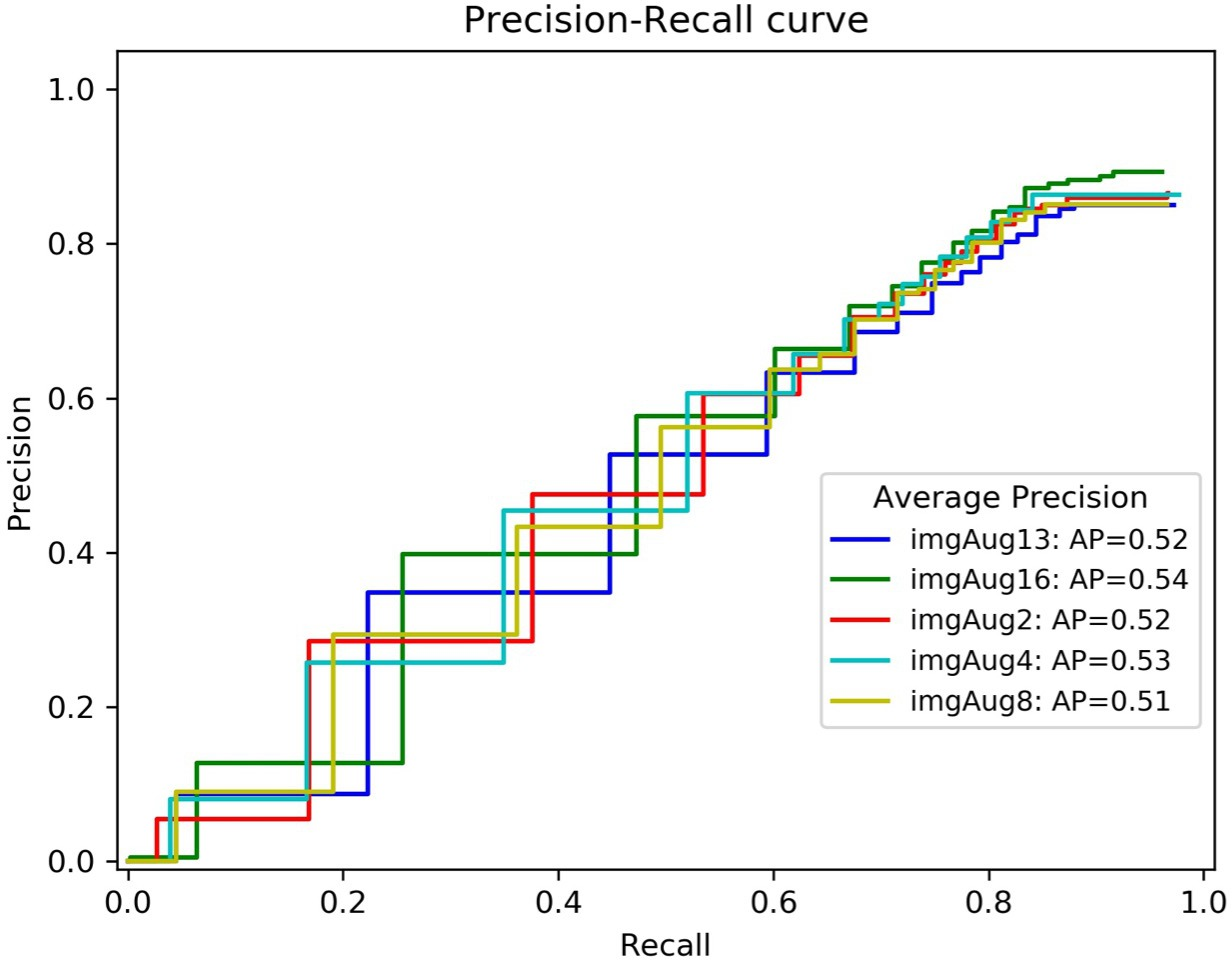
\includegraphics[width=10cm]{figures/top5_curves_trim.jpg}
	\caption{Precision-recall curves of the top five average precision (AP) in experiments of data augmentation (labeled as ``imgAugX", where X is the experiment number).}
	\label{fig_ap_top5}
\end{figure}

\begin{figure}
	\centering
	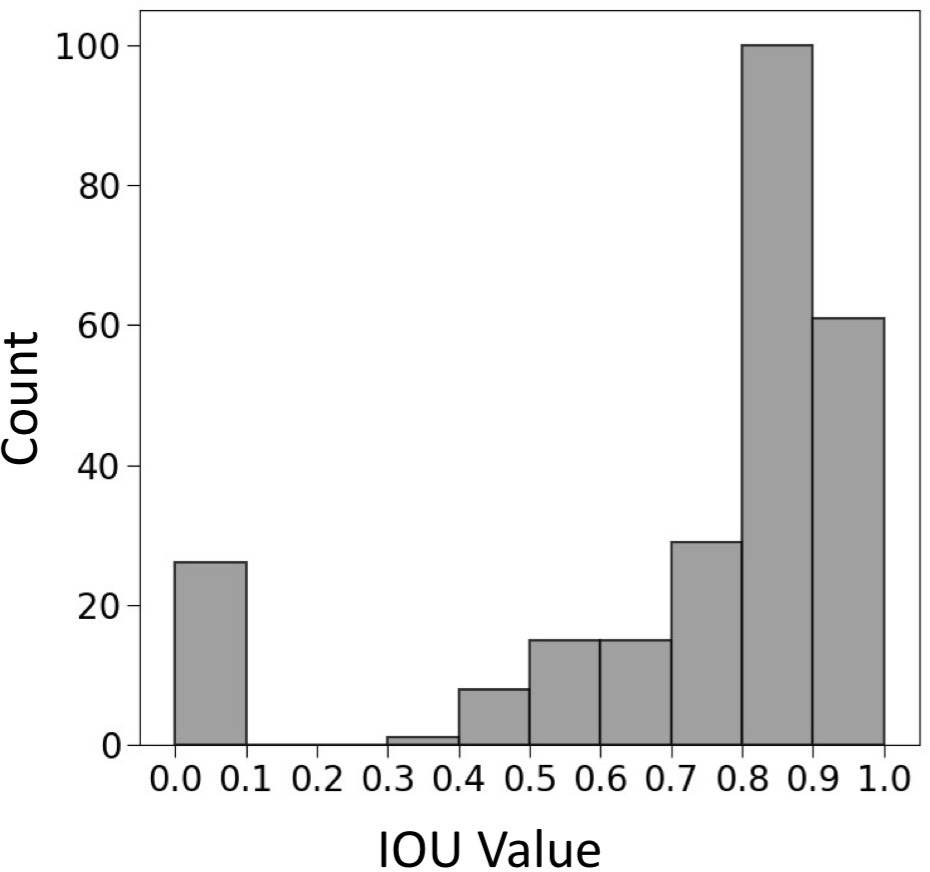
\includegraphics[width=8cm]{figures/IoU_imgAug22_label_trim.jpg}
	\caption{IOU histogram of the mapped polygons in experiment \#22.}
	\label{fig_iou_hist_exp16}
\end{figure}

\subsection{Mapped polygons and their accuracies}
\label{subsec_mapped_accuracies}

There are \replaced{255}{196}\added{ (TP+FP)} mapped polygons in experiment \#\replaced{22}{16}, as shown in Table \ref{table_acc_imgaug}, which has the highest AP.  Fig. \ref{fig_mapped_rts} and \ref{fig_zoomin_mapped_rts} show their spatial distributions and the corresponding amplifications of selected regions. With an IOU threshold of 0.5, which is commonly used, \replaced{220}{165} of them are true positives, \replaced{35}{31} are false positives, and \replaced{44}{37} of the ground truths are missed, i.e., false negatives. The corresponding precision, recall, and F1 score are \replaced{0.863, 0.833, and 0.848}{0.842, 0.817, and 0.829}, respectively. \deleted{For the pixel-based validation, the Kappa index is 0.917 and the overall accuracy index is 0.999.}As shown in Fig. \ref{fig_zoomin_mapped_rts}, the automatic-based boundaries match the manual-based ones very well, consistent with Fig. \ref{fig_iou_hist_exp16}, which shows that most of the IOU values are greater than 0.7. The false positives are at the locations where the land covers are similar to the RTSs. Since some of the RTSs are close to each other (their closest part is less than 15 m, i.e., five pixels), they were merged into one RTS,
% by the mapping method, 
so that the sum of TP and FN is not equal to the number of ground truths in some experiments (see Table S1). Once a mapped polygon covers two or more RTSs, it would be categorized as a true positive if its IOU value is greater than 0.5, otherwise as a false positive (examples of true and false positives are marked by red and yellow rectangles in Fig. \ref{fig_zoomin_mapped_rts}a, respectively). 
%In experiment \#16, there are 17 mapped polygons, each of which covers more than two RTSs and cover 37 RTSs in total. 

%Polygon-based validation is more practical and understandable than pixel-based validation. We achieved a very high overall accuracy index (i.e., 0.999) because most of the study area are non-RTS, and was corrected labeled as non-RTS pixels. The pixel-based are suitable for comparison with other methods which conduct classification pixel by pixel. However, our targets are the extents of RTSs. Therefore, polygon-based validation is more suitable and meaningful for this study.

\begin{figure}
	\centering
	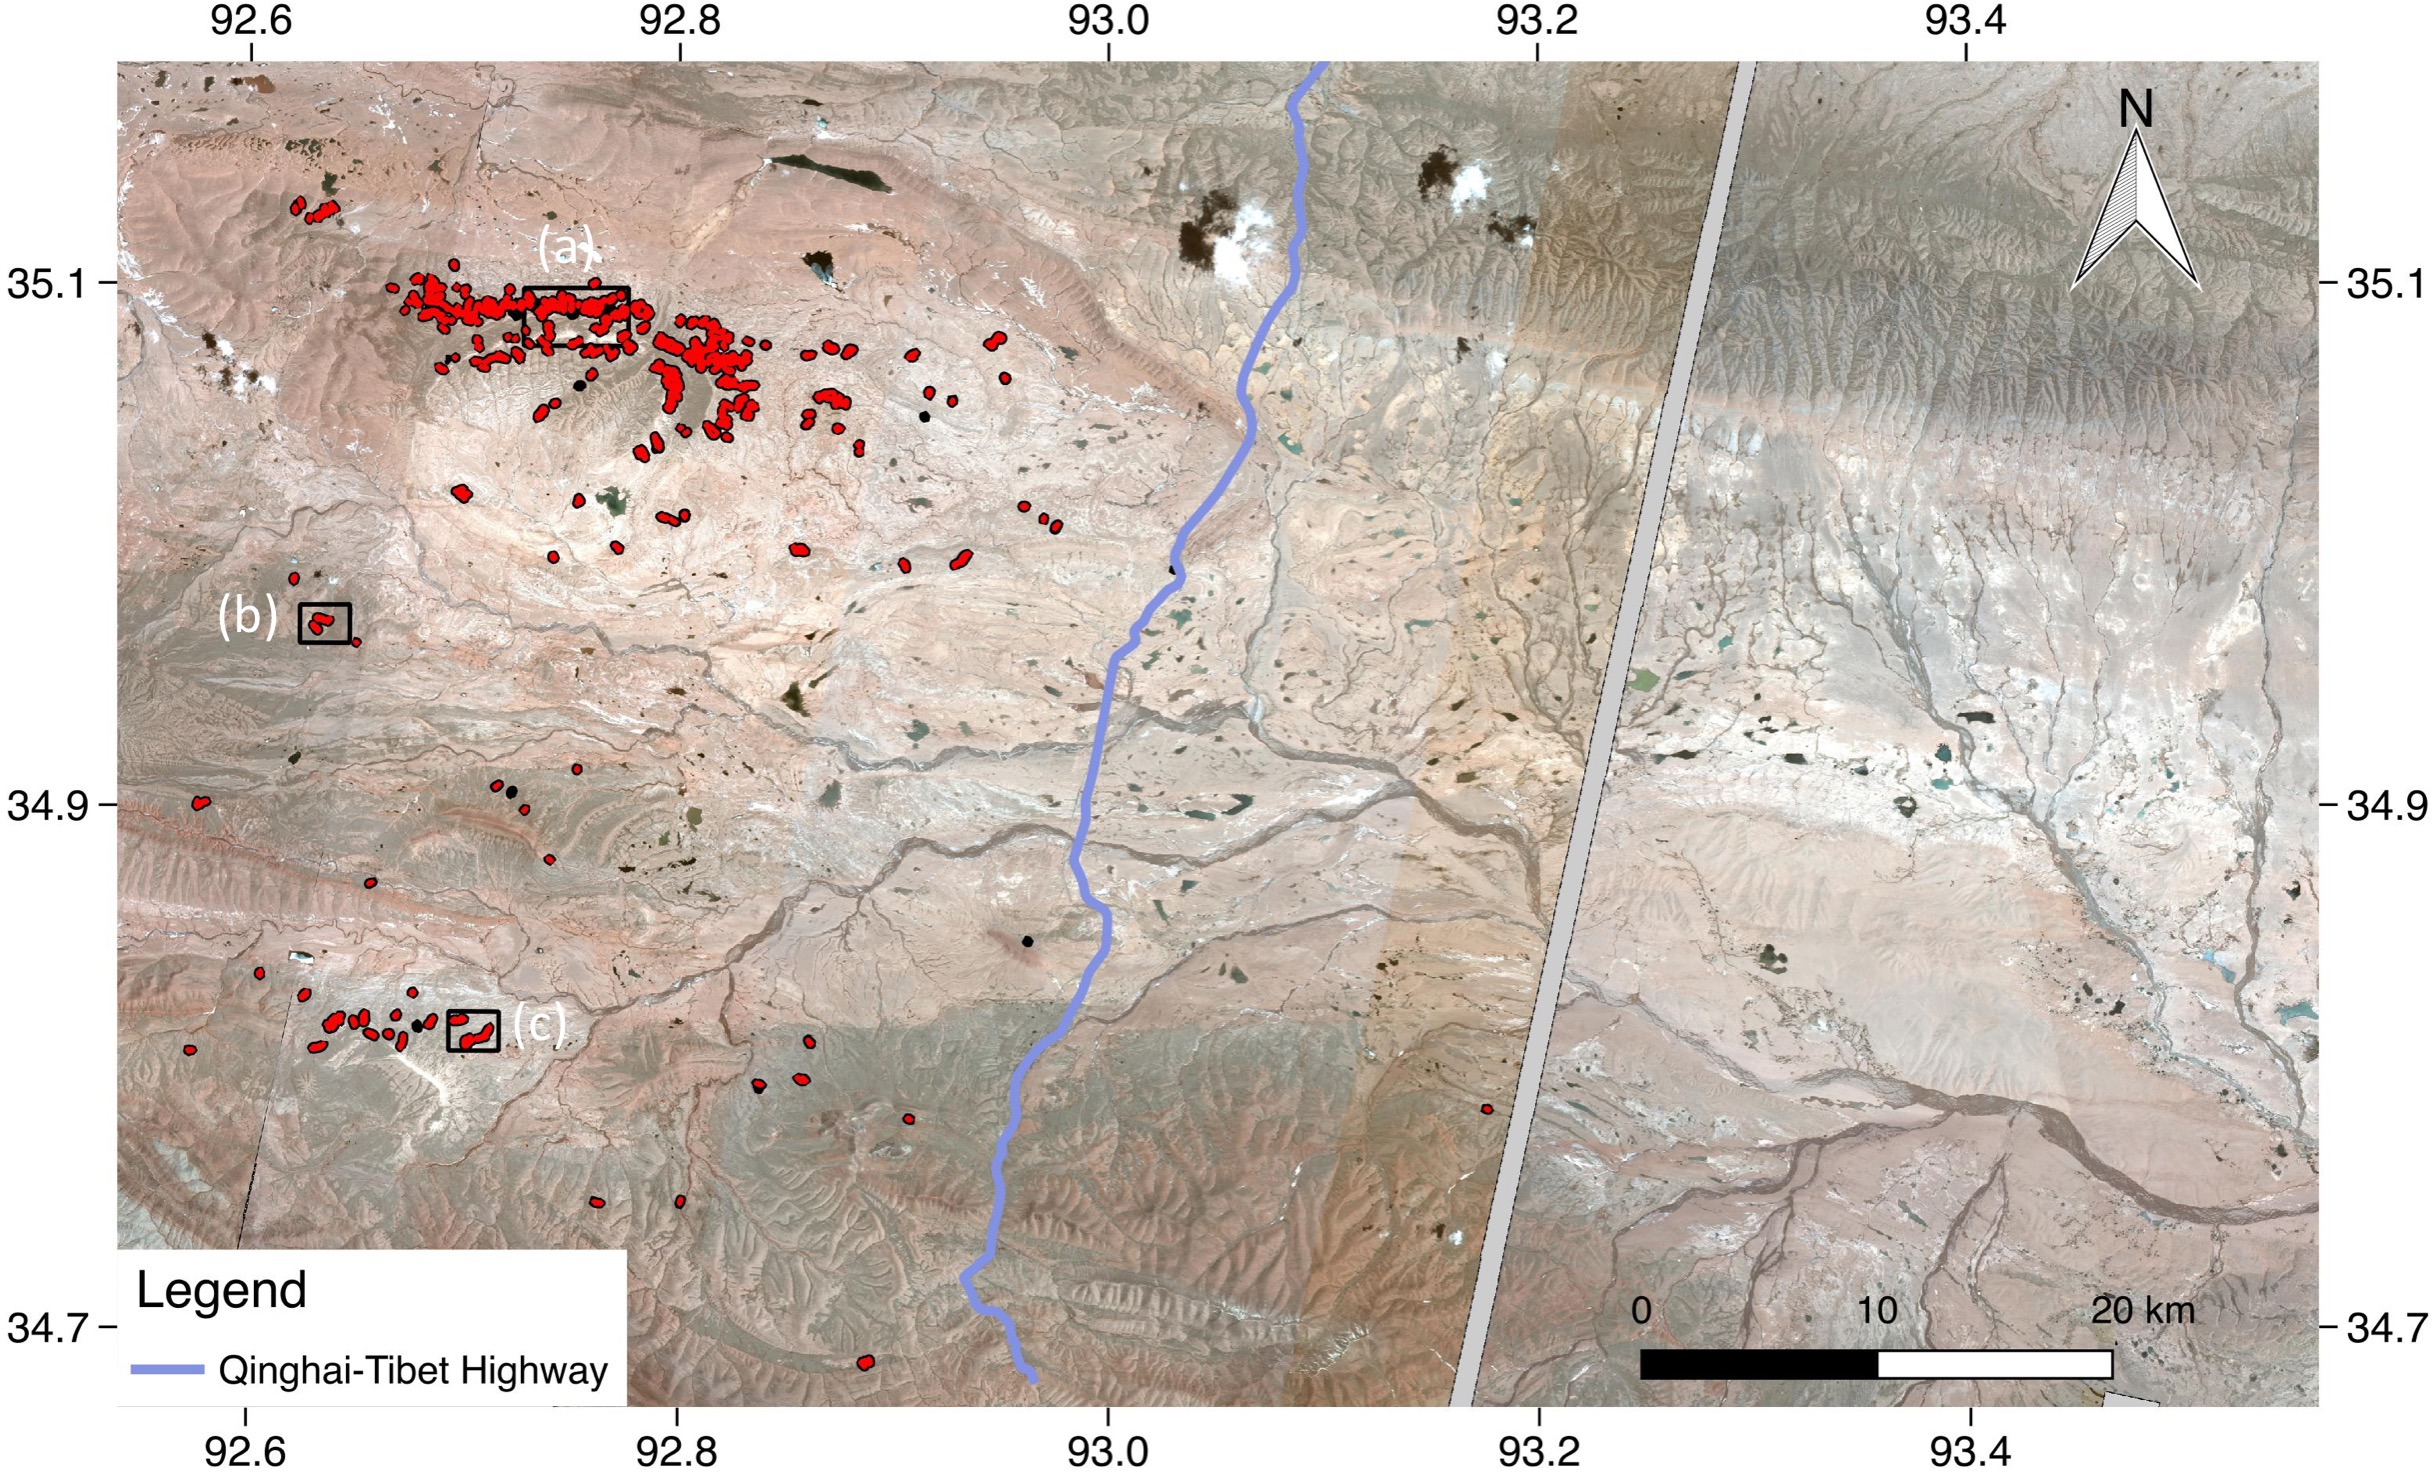
\includegraphics[width=14cm]{figures/whole_area_mapped_trim.jpg}
	\caption{Automatically mapped retrogressive thaw slumps (red polygons) versus manual delineation (black polygons) on Planet images. The red polygons are true positives of the mapped polygons in Experiment \#\replaced{22}{16}. (a)--(c) are extents of the figures in Fig. \ref{fig_zoomin_mapped_rts}. The grey gap is due to the lack of Planet scenes.}
	\label{fig_mapped_rts}
\end{figure}

\begin{figure}
	\centering
	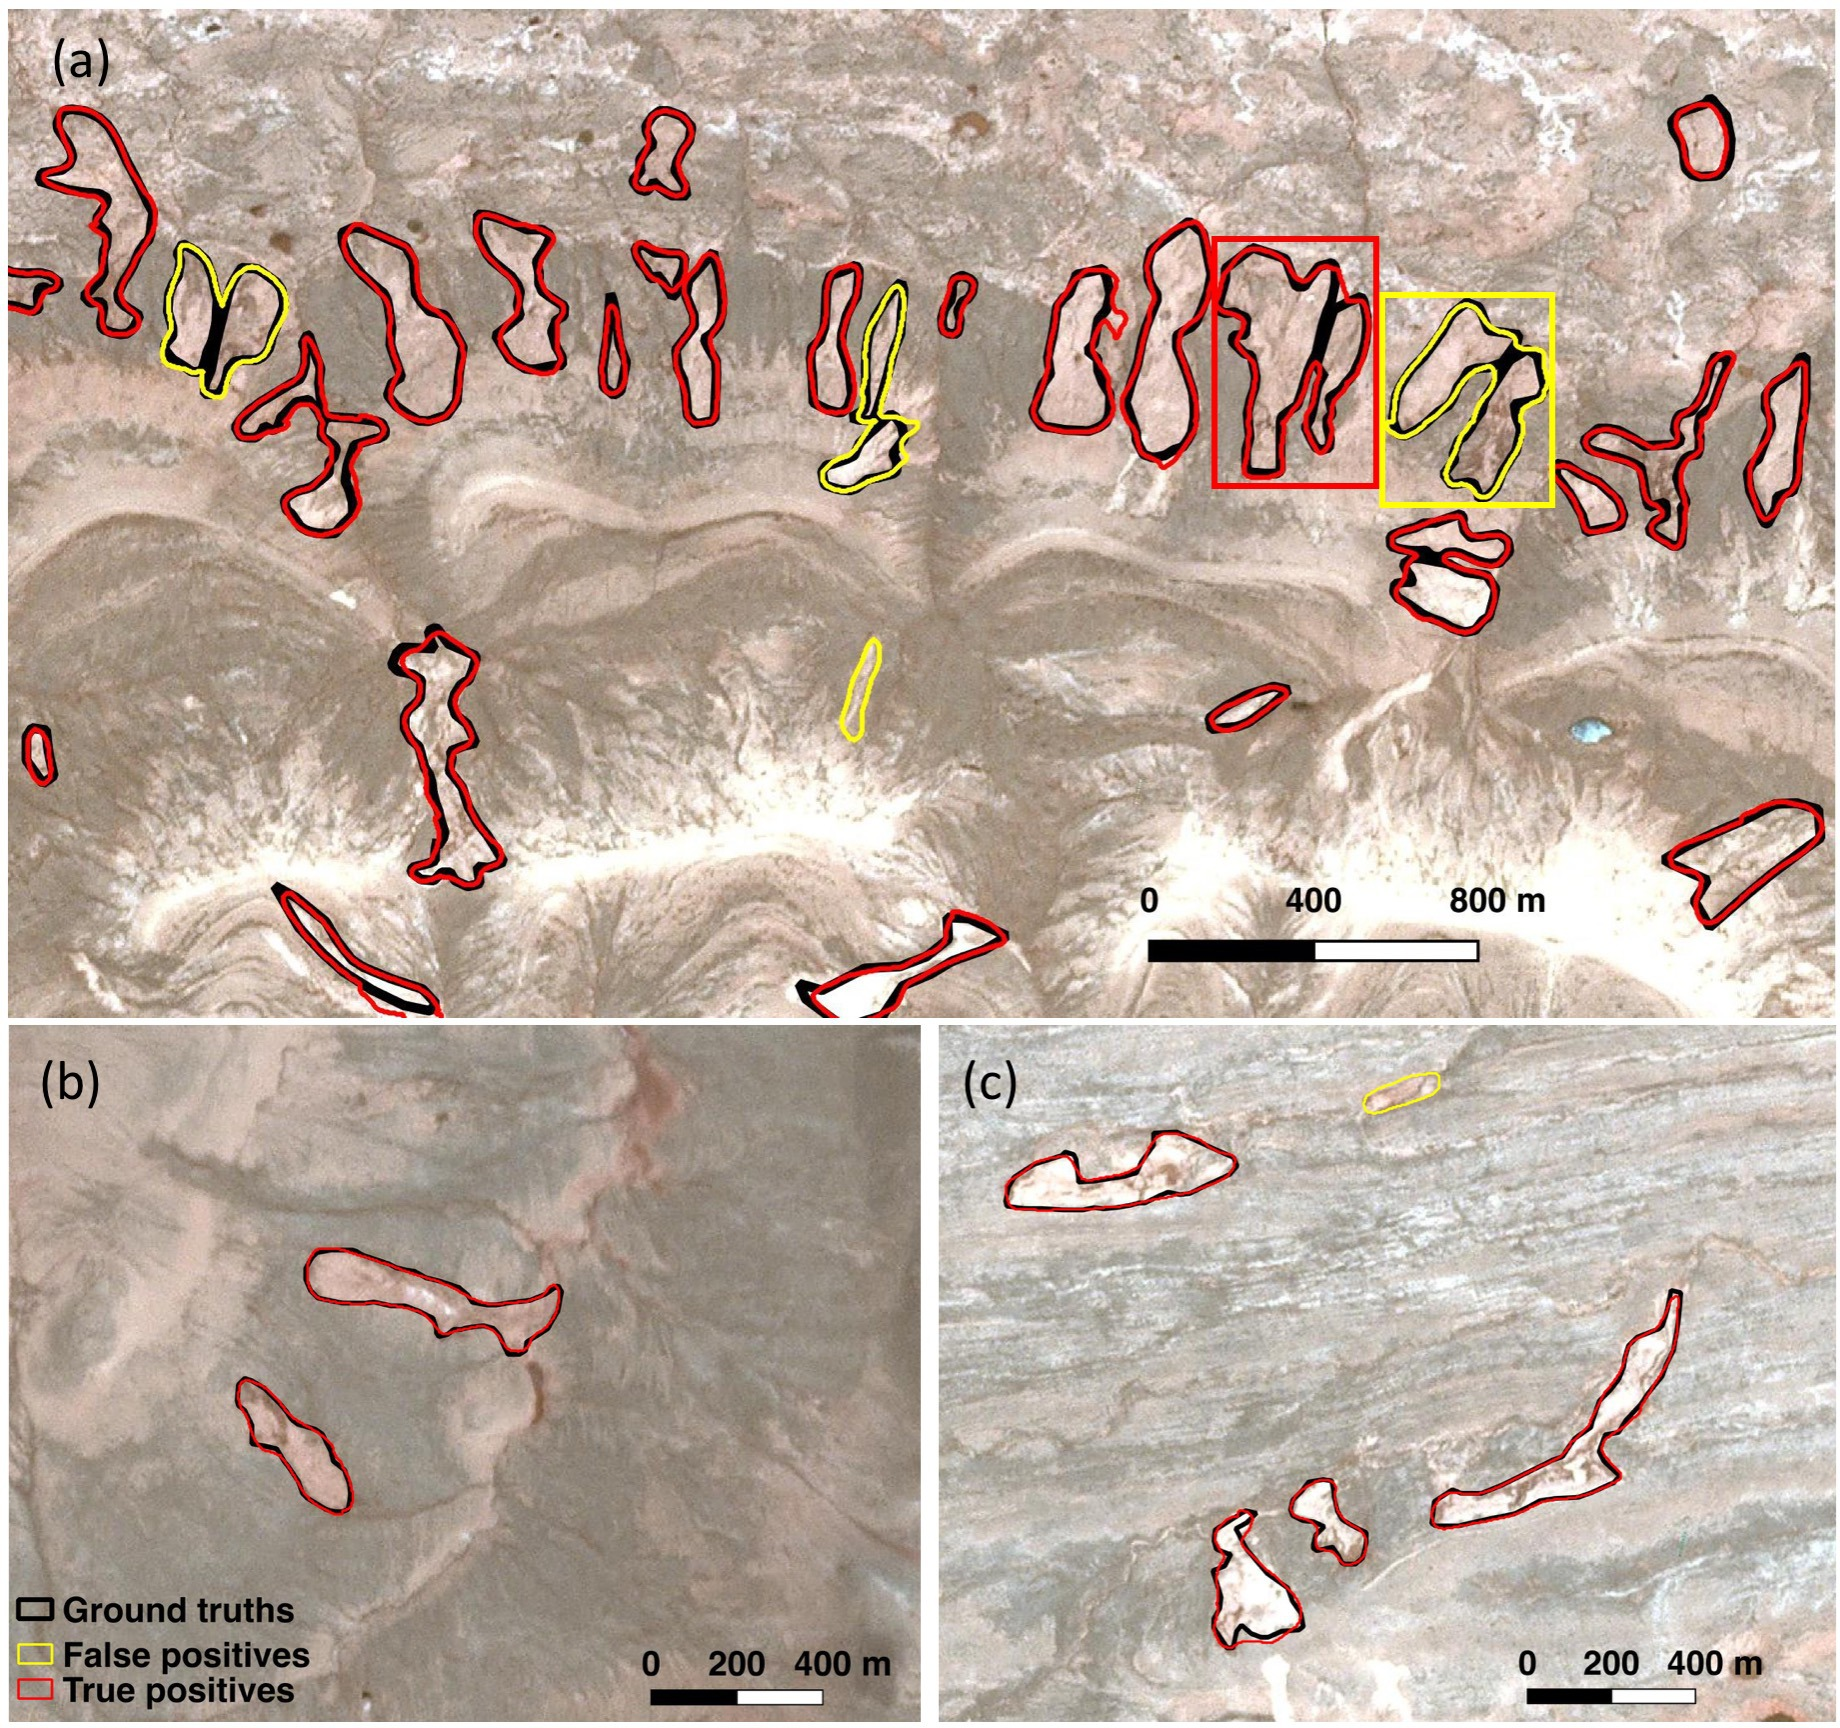
\includegraphics[width=12cm]{figures/zoom_in_mapped_polygons_trim.jpg}
	\caption{Amplifications of mapping results. (a)--(c) are amplifications of three regions marked by black rectangles in Fig. \ref{fig_mapped_rts}. The two rectangles marked are discussed in sections \ref{subsec_mapped_accuracies} and \ref{subsec_advantage_limitation_method}.}
	\label{fig_zoomin_mapped_rts}
\end{figure}


\subsection{Generalization of the trained model in a test area}
\label{subsec_newArea}
% result in a distinct geographic regions
% Test accuracies in a new area?

\added{The prediction in a test area achieves good accuracies by using the trained model in experiment \#22. 
The area has a size of approximately 4000 km$^2$ and is to the northwest of our study area, as shown in Fig. S15a in the Supplementary Materials. 
It was chosen randomly because we did not know RTS distribution outside the Beiluhe region. 
The objective of this prediction test is to evaluate the generalization of trained models. 
The input image is a mosaic of 47 Planet images acquired on 22 and 23 May 2018. 
The network model for prediction was trained using the training data collected in Beiluhe and the setting of experiment \#22. 
As shown in Fig. S15b and S16, the trained model delineated 62 mapped polygons. 
For validation, we used the same method as described in section \ref{subsec_collect_groundtruth} to manually delineate RTSs in this area and obtained 50 RTS polygons as ground truths. 
With the IOU threshold of 0.5, TP, FP, and FN are 33, 20, and 17, respectively. 
Therefore, the precision, recall, and F1 score are 0.532, 0.660, and 0.589, which demonstrates the good generalization of the trained model in the test area.}

\added{The accuracy in the test area is lower than the one in Beiluhe. 
A comparison between results in Beiluhe (Tables \ref{table_acc_imgaug} and S1) and the test area shows that (1) the F1 scores in Beiluhe are higher by around 0.2 and (2) IOU values (Fig. S17) of mapped polygons are lower than the ones in Beiluhe. 
The lower IOU values indicate that the mapped polygons match the ground truths but not as well as the case in Beiluhe, as exampled in Fig. S16a and b. 
The reason for the lower F1 score in the test area is that some of the RTSs or land cover with different appearances on the images were not included in the Beiluhe training data. 
For example, Fig. S16c shows two false negatives which are darker than most RTSs in Beiluhe on the Planet images. 
Fig. S16a and d show examples of false positives which have similar appearances of RTSs in Beiluhe. 
Fig. S16e presents a case that the mapping method only picked a portion of an RTS, indicating that the features of this RTS are not well learned by the trained model.}

%mark a line here 
%We only conduct one experiment in the test areas because others expeirment would be similar. 


\subsection{Improvement due to data augmentation}
\label{subsec_contrib_dataAug}

A comparison between the experiments with and without data augmentation shows that including data augmentation can improve the IOU values of mapped polygons. \deleted{ but introduce more false positives.} The F1 scores of experiment \#0 at IOU thresholds of 0 and 0.4 are close to those obtained in other experiments, and the difference between them is within \replaced{0.08}{0.05}. 
%The difference between them is smaller than 0.05. 
However, when the IOU threshold is 0.8, the difference increases significantly to \replaced{0.15}{0.17} (comparing \#0 and \#\replaced{26}{16}). Moreover, all the experiments with data augmentation, except \#5\added{, \#9, and \#15} have higher F1 scores than \#0. \added{Moreover, a comparison between Fig. \ref{fig_iou_hist_exp16} and S14 shows that the number of mapped polygons with IOU values greater than 0.9 increases dramatically after applying data augmentation.} Therefore, data augmentation increases the IOU values, namely, the mapped polygons better match the ground truths. \replaced{Some of the experiments (i.e., \#5, \#9, and \#15) are}{Experiment \#5 is a} particular case\added{s}\deleted{ in point}, since rotating produced more false negatives. 
%As shown in Table \ref{table_acc_imgaug}, 
\deleted{Lastly, experiment \#0 has a relatively small number of false positives (17), which implies that the data augmentation also leads to more false positives. }


Different data augmentation methods may make different contributions to improving accuracies. Table \ref{table_stastic_imgaug} lists the statistics on the minimum, maximum, and average of F1 scores at different IOU thresholds when adopting different data augmentation methods. 
\added{In the 31 experiments with data augmentation (Table S1), each method was adopted in 16 experiments. }
When the IOU threshold is 0.8, there is a difference of F1 scores between experiments adopting rotating and other methods. The difference decreases when the IOU threshold is 0.4 and becomes negligible when it is zero. 


\begin{table}[ht]
\centering
\footnotesize
\caption{Statistics of accuracies based on different data augmentation methods.}
\label{table_stastic_imgaug}
%\centering
%% \tablesize{} %% You can specify the fontsize here, e.g. \tablesize{\footnotesize}. If commented out \small will be used.
%\begin{tabular}{cc m{2.2cm}  m{2.2cm}  m{2.2cm} ccc}
\begin{tabular}{c c c c  c  }
\toprule
\multirow{2}{*}{\textbf{IOU}}&\multirow{2}{*}{\textbf{Methods}}& \multicolumn{3}{c}{ \textbf{F1 score}} \\
 & &\textbf{min}&\textbf{max}&\textbf{mean}\\
\midrule
\multirow{5}{*}{0.8} & F &     0.479 & 0.634 & 0.575 \\
&      B & 0.507 & 0.634 & 0.572 \\
&      C & 0.522 & 0.634 & 0.582 \\
&      S & 0.447 & 0.634 & 0.571 \\
&      R & 0.410 & 0.586 & 0.530 \\

\midrule
\multirow{5}{*}{0.4}&      F & 0.801 & 0.863 & 0.841 \\
&      B & 0.826 & 0.885 & 0.847 \\
&      C & 0.801 & 0.885 & 0.849 \\
&      S & 0.801 & 0.885 & 0.844 \\
&      R & 0.801 & 0.859 & 0.833 \\

\midrule
\multirow{5}{*}{0.0} &     F & 0.857 & 0.921 & 0.895 \\
&      B & 0.877 & 0.935 & 0.902 \\
&      C & 0.857 & 0.935 & 0.900 \\
&      S & 0.857 & 0.935 & 0.898 \\
&      R & 0.857 & 0.928 & 0.890 \\

%F: flipping, B: blurring, C:cropping, S:scaling, R: rotating

\bottomrule
\end{tabular}
\end{table}

\subsection{Other combinations of the four bands of Planet images}
\label{subsec_otherbands}

The combination of red, blue, and green bands outperforms other combinations.
% as shown in Table \ref{table_acc_otherbands}. 
Table \ref{table_acc_otherbands} lists the accuracies of two experiments, which also adopted data augmentation of \replaced{scaling}{flipping}, blurring, and cropping. The band combination of experiment \#32 is the blue band of Planet images, NDVI, and NDWI. Experiment \#33 utilized the first three PCA \replaced{bands}{components}. All the experiments listed in Table \ref{table_acc_imgaug} and S1 used the RGB bands. Compared to the experiments using RGB bands, experiment \#32 \added{and \#33} achieved \added{relatively low APs.} \deleted{a good AP but not the highest, while experiment \#33 obtained the lowest AP.} Possible reasons are (1) the training polygons were delineated on RGB images, which make the features utilized in the manual delineation and automatic mapping consistent, (2) the vegetation in the study area is sparse, so the changes in NDVI are small, (3) on the surface, water content is very high or the soil is saturated during the thaw season, which lowers the effectiveness of NDWI, and (4) after PCA, some key features for identifying RTSs may disappear. 

\begin{table}[ht]
\footnotesize
\caption{Accuracies of other band combinations.}
\label{table_acc_otherbands}
%\centering
%% \tablesize{} %% You can specify the fontsize here, e.g. \tablesize{\footnotesize}. If commented out \small will be used.
%\begin{tabular}{cc m{2.2cm}  m{2.2cm}  m{2.2cm} ccc}
\begin{tabular}{c c c c  c ccc c c c c}
\toprule
\textbf{\#}&\textbf{Bands}&\textbf{AP}&\textbf{IOU}&\textbf{TP}&\textbf{FP}&\textbf{FN}&\textbf{Pre}&\textbf{Rec}&\textbf{F1}\\
\midrule

\multirow{3}{*}{32} &  \multirow{3}{3cm}{Blue, NDVI, NDWI} & \multirow{3}{*}{0.493}  &0.8&162   & 103   & 101   & 0.611  & 0.616  & 0.614   \\
 &  &  &0.4&221   & 44    & 40    & 0.834  & 0.847  & 0.840 \\
 &  &  &0.0&225   & 40    & 14    & 0.849  & 0.941  & 0.893   \\
 
\midrule

\multirow{3}{*}{33} &  \multirow{3}{3cm}{1--3 bands after PCA} & \multirow{3}{*}{0.474} &0.8& 158   & 96    & 105   & 0.622  & 0.601  & 0.611  \\
 &  &  &0.4& 209   & 45    & 52    & 0.823  & 0.801  & 0.812  \\
 &  & &0.0& 217   & 37    & 23    & 0.854  & 0.904  & 0.879  \\

\bottomrule
\end{tabular}

%\raggedright \#: the continuous experiment number
\end{table}



\subsection{Factors affecting the accuracies}
\label{subsec_acc_factors}

The IOU value, which represents the delineated accuracy of an individual RTS, can be affected by the geometric characteristics of RTSs.
The delineated accuracies are critical for analyzing the temporal change of RTS extents and the total mapping accuracies.
%In this study, we analyzed the relations between IOU values and geometric characteristics of RTSs as well as the count of adjacent RTSs.
Fig. \replaced{S9 and S10}{S8 and S9} in the Supplementary Materials are scatter plots between IOU values and areas as well as perimeters. They show that a small mapped polygon (whose area and perimeter are smaller than most of the polygons) tends to have lower IOU values, but there are also many mapped polygons with high IOU values are small in size. 
\added{The possible reason for the small mapped polygons with high IOU values is that they shared similar features which were enhanced during training and were easier to be detected during prediction.}
%If the mapped polygons have a larger size, they tend to have higher IOU values.
The IOU values do not correlate with the circularities of RTSs as shown in Fig. \replaced{S11}{S10} in the Supplementary Materials. 


As shown in Fig. \replaced{S12}{S11} in the Supplementary Materials, the count of adjacent RTSs can affect the IOU values. The adjacent RTSs are those RTSs which have intersections with the buffer area of a central RTS. Fig. \replaced{S12}{S11} only shows the mapped polygons which cover a single RTS. The false positives are those with zero or two adjacent RTSs, and the zeros are the majority. Many high IOU values also occur where the count of the adjacent RTSs is zero. The reason could be that these RTSs share similar features which are enhanced during training. The setting of buffer areas and overlap pixels in the step of preparation of training images results in the duplication of RTS pixels. If an RTS has more adjacent RTSs, it would have more duplications in the training data. Therefore, the deep learning algorithm learns more features of the RTS and is more sensitive to both it and similar ones. 

The uncertainty of the training polygons, some of which are derived from ground truths, could also have affected the mapping accuracies. The possible uncertainties include: (1) RTSs may have been at different stages of development, but we did not distinguish between them when collecting and validating the ground truths; (2) many of the RTSs were validated in 2014, but the images were only acquired in 2018; and (3) around \replaced{30}{10}\% of ground truths were used without validation in the field. 


\section{Characteristics of RTSs and their terrain factors}
\label{sec_spatial_terrain}


\subsection{Geometric characteristics of RTSs}
\label{subsec_geo_charac}

\begin{figure}
	\centering
	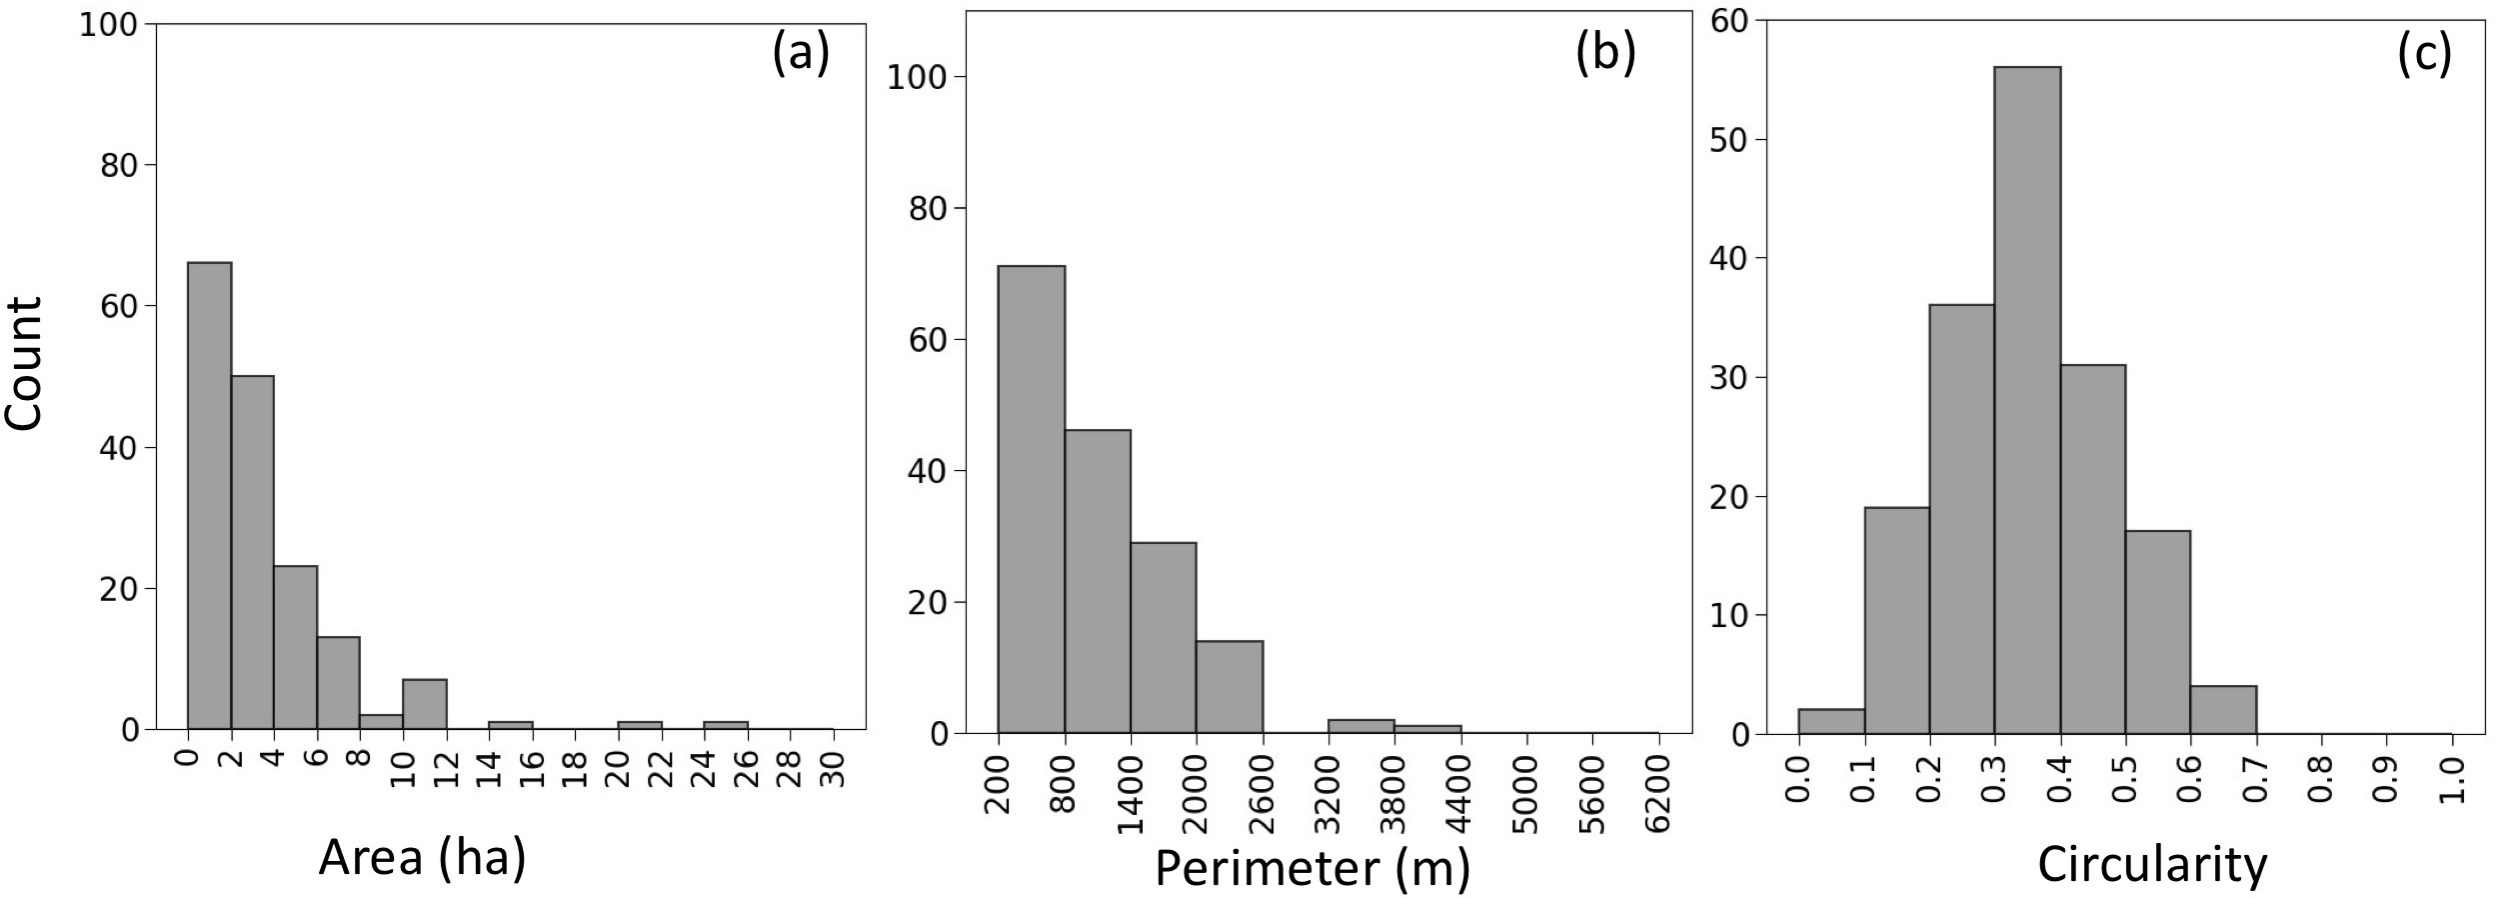
\includegraphics[width=14cm]{figures/geometric_var_mapped_trim.jpg}
	\caption{Geometric statistics of the RTSs based on mapped RTSs of experiment \#22 in Table \ref{table_acc_imgaug}. One RTS whose area is \replaced{35.2}{34.6} ha not shown in (a), and two RTSs, whose perimeters are \replaced{6972}{6924} meters and \replaced{8910}{8226} meters, respectively, are not shown in (b) because they are out of range. }
	\label{fig_geometric_statistics}
\end{figure}


Fig. \ref{fig_geometric_statistics} shows the geometric characteristics of mapped RTSs.  The areas of the mapped RTSs range from 0.3 to \replaced{35.2}{34.6} ha, with an average of \replaced{3.5}{3.7} ha, and \replaced{93}{95}\% of them are smaller than eight ha (Fig. \ref{fig_geometric_statistics}a). Their perimeters range from \replaced{270}{288} to \replaced{8910}{8226} meters, with an average of \replaced{1158}{1191} meters, and 90\% of them are smaller than 2000 meters \added{in length} (Fig. \ref{fig_geometric_statistics}b). Fig. \ref{fig_geometric_statistics}c shows a nearly normal distribution of the circularities with minimum, maximum, and average of 0.06, \replaced{0.63}{0.65}, and \replaced{0.34}{0.35}, respectively. 

The geometric characteristics of the mapped RTSs are similar to those \replaced{featured in the ground truth dataset}{ featuring as ground truths}. Fig. \replaced{S7}{S6} in the Supplementary Materials shows that the averages of the areas, perimeters, circularities of the ground truths 
%range from 0.25 to 28.3 ha, 235 to 5898 meters, and 0.1 to 0.9, respectively. Their averages
 are \replaced{3.0}{3.1} ha, \replaced{881}{893} meters, and 0.49, respectively. The averages of the areas and perimeters of the mapped RTSs are higher than those of the ground truths, but the average circularity is lower. These differences are possibly due to the fact that (1) many small and nearly circular RTSs were missed in the mapped results and (2) some of the RTSs are close to each other and may have \added{been} merged into a single polygon, such as the one marked by the red rectangle in Fig. \ref{fig_zoomin_mapped_rts}a.  

\subsection{Terrain factors of RTSs}
\label{subsec_terrain}

\begin{figure}
	\centering
	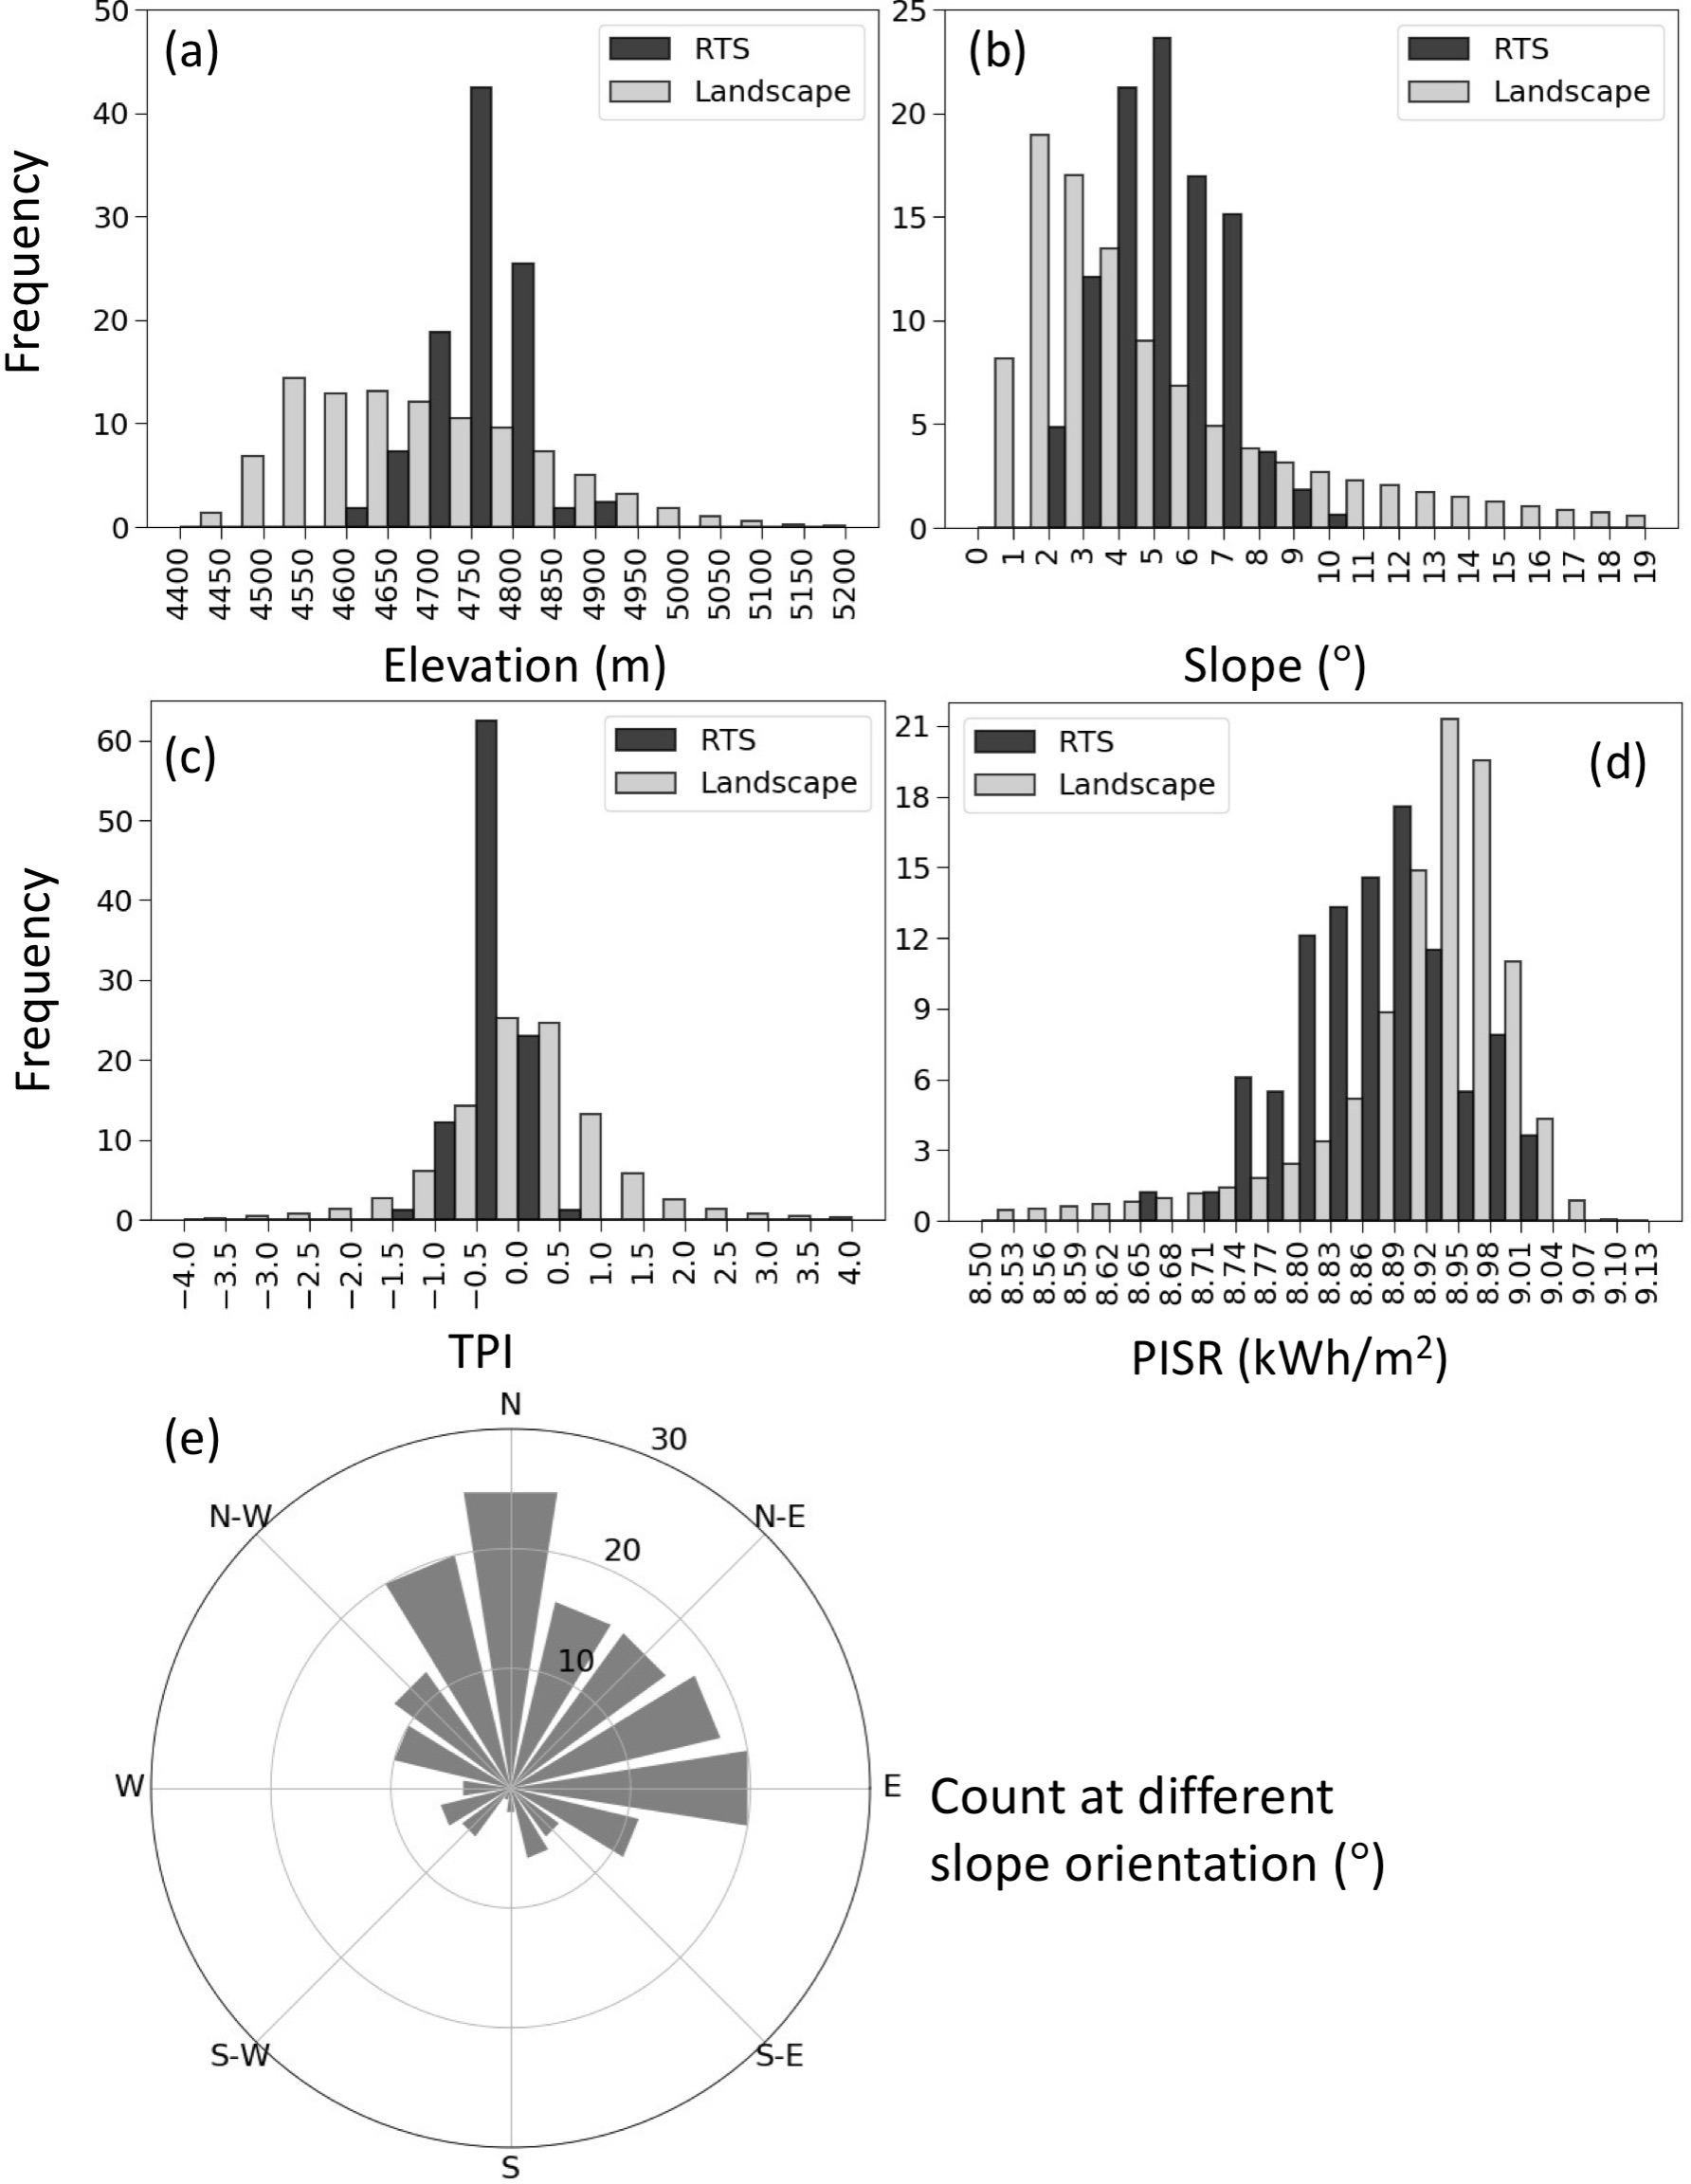
\includegraphics[width=13cm]{figures/terrain_var_fig_mapped_trim.jpg}
	\caption{Statistics of RTS terrain factors based on automatic mapping results  (\#22 in Table \ref{table_acc_imgaug}). Landscape refers to the entire study area.}
	\label{fig_terrain_factors}
\end{figure}

Fig. \ref{fig_terrain_factors} shows the statistics of the mapped RTSs in different ranges of terrain factors. Their elevation and slope range from \replaced{4552}{4639} meters to 4938 meters and from 2.4 degrees to \replaced{12.1}{10.2} degrees, with an average of \replaced{4768}{4776} meters and \replaced{5.5}{5.6} degrees, respectively. Fig. \ref{fig_terrain_factors}a and b show that RTSs preferentially occur at elevations from 4700 to 4850 meters, and on slopes from four to eight degrees. The TPI of mapped RTSs range from $-1.3$ to 0.6, with an average of $-0.17$ (Fig. \ref{fig_terrain_factors}c), indicating that most of the RTSs were initiated at a location slightly lower than their surroundings, although they are still on the slopes. \added{The possible reasons will be given in section \ref{subsec_rts_spatial}.} Their daily PISR of the RTS locations in summer varies from \replaced{8.72}{8.65} to 9.04 $kWh/m^2$, with a mean of \replaced{8.89}{8.88} $kWh/m^2$. The PISR of the entire area is between 8.50 and 9.13 $kWh/m^2$, with a mean of 8.91 $kWh/m^2$. Fig. \ref{fig_terrain_factors}d shows that RTSs preferentially occur at locations where the PISR ranges from 8.74 to \replaced{9.01}{8.92} $kWh/m^2$.
%, which less than the majority landscapes. 
The preferential orientations of the mapped RTSs are north and northeast (Fig. \ref{fig_terrain_factors}e), so that they tend to receive less incoming solar radiation than those oriented southwards. 

A comparison between Fig. \ref{fig_terrain_factors} and Fig. \replaced{S8}{S7} in the Supplementary Materials shows that there is no significant difference in occurrences between mapped RTSs and ground truths. The averages of elevation, slope, TPI, and PISR based on the ground truths are \replaced{4770}{4775} meters, \replaced{5.6}{5.7} meters, \replaced{$-0.16$}{$-0.15$}, and \replaced{8.89}{8.88} $kWh/m^2$. The distributions of slope orientations are similar except that the total number is reduced because some RTSs have been missed in the mapped results. 

\subsection{Spatial distribution and the terrain controlling factors}
\label{subsec_rts_spatial}

Most of the RTSs are in the western, particularly the northwestern section, of the study area. As shown in Fig. \ref{fig_mapped_rts}, there is a cluster of RTSs in the northwestern region. Most of the RTSs in this cluster are on the north-facing slope of a mountain. \added{In our study area, north-facing slopes are cooler than south-facing ones because they received less direct solar radiation throughout the year.} Many RTSs are isolated to the west of the Qinghai-Tibet Highway. There is only one RTS to the east of the highway. Many factors, including vegetation, soil texture, and ice context, can affect the spatial distribution of RTSs, as well as permafrost, but these elements are beyond the scope of this study. The relationships between RTS spatial distribution and terrain factors, including elevation, slope angle as well as orientation, TPI, and PISR are discussed as follows.

%Many factors such as vegetation and soil types relating to permafrost distribution as described in \citealp{yin2017effects} can also affect the spatial distribution RTSs. 


%\subsection{Relation between the RTS spatial distribution and terrain factors}
%\label{subsec_spatial_dis_terrain}


%The elevation is the main factor affecting the spatial distribution of RTSs. 
In this area, RTSs are distributed in the locations which have a relatively high elevation.
As shown in Fig. \ref{fig_mapped_rts}, almost all the RTSs are to the west of the Qinghai-Tibet Highway, at a higher elevation to those located east of the highway, as shown in Fig. \replaced{S13}{S12} in the Supplementary Materials. Permafrost on the Tibetan Plateau is known as Plateau Permafrost, as its formation is mainly controlled by the elevation of the land. Therefore, elevation affects the spatial distribution of permafrost, thereby also limiting the spatial distribution of RTSs. However, elevation is not the only factor controlling the distribution of permafrost. As a previous study has highlighted, other factors such as vegetation, \added{aspect}, and soil types can also affect its distribution \citep{yin2017effects}.

RTSs tend to occur on gentle slopes, a tendency which has been been noted in many previous studies (e.g., \citealp{leibman1995cryogenic, niu2014thaw, lacelle_distribution_2015}). Slope condition is important, because water and melted materials from permafrost flow downward and keep the permafrost exposed to the air. In permafrost areas, a gentle slope allows water to accumulate under the active layer. The accumulation of water reduces the friction between the uppermost permafrost and the active layer,  then triggers the detachment of the active layer and exposes the ice-rich permafrost \citep{mcroberts1974stability, mcroberts1974the}. \added{Once ice-rich permafrost is exposed, the solar radiation can warm it directly, then cause a rapid thawing.}

The TPI statistics show that RTSs are common in locations that are lower than their surroundings. The lower position allows water from the melting of ground ice or precipitation to easily accumulate, making it more likely to trigger the detachment of active layers. Lower positions tend to accumulate snow from precipitation and wind blow in winter. Snow cover can prevent the cooling of permafrost in the winter, which increases the likelihood that the permafrost will thaw in the next thaw season \added{\citep{stieglitz2003role}}. 

Slope orientation and PISR consistently show that RTSs preferentially exist at locations receiving less solar radiation. Less solar radiation can lead to shallower active layers, which increase the likelihood of ground ice being closer to the surface and hence more accessible to thawing. North-facing slopes may have greater snow accumulation and persistence, which can increase the soil moisture in the thaw season. \deleted{More RTSs are on east-facing slopes than those facing west, because convective clouds are commonly found between noon and 6 pm local time
%, which results in higher insolation in the morning 
\text{\citep{niu2014thaw}}.}


\section{Discussion}
\label{sec_discussion}

\subsection{Advantages and limitations of using Planet CubeSat images}
\label{subsec_advantage_limitation_planet}

Global coverage and high temporal resolution are some of the advantages of using Planet images. RTSs are the most striking dynamic landforms in the permafrost, and images with a high temporal resolution are required to monitor their temporal changes. The images from the similar sensors aboard the Planet CubeSats make the pre-processing and analysis of images a simple task with fewer uncertainties. With the advantage of high temporal resolution, we can track the highly dynamic changes of the earth's surface. 
%Planet also provides the monthly mosaic of cloud-free images but only available for commercial request. 
The global coverage of Planet images makes it easy to extend our method to other regions for mapping RTSs without re-training. 

The spatial resolution of Planet images is the main limitation, which results in the loss of many small (less than 0.3 ha) \added{and obscure} RTSs in the results. Although the Planet images have a nominal spatial resolution of 3.0 meters, their actual resolution can be lower depending on the parameters of CubeSat, such as looking angles.
% and \hl{one more parameter?}. 
RTSs contain many portions including headwall, slump floor, and slump lobe. It may not be possible to distinguish between the different portions of RTSs, even those with an area greater than 0.3 ha. Moreover, if the temporal changes of the RTS are smaller than one pixel of Planet images, then they cannot be identified. Most of the stabilized thaw slumps are drier and covered by new vegetation, much like their surroundings, which makes it challenging to identify them. 
\added{Therefore, we may have missed some RTSs when manually delineated them on Planet images.}
% although Planet images have four bands.

\subsection{Advantages and limitations of the automatic mapping method}
\label{subsec_advantage_limitation_method}

The automatic mapping method can potentially be applied to a large area such as the Tibetan Plateau, and allows us to map RTSs to an unprecedented extent. Many permafrost areas remain unmapped because (1) they are challenging to reach and (2) manually mapping on high-resolution images is labor-intensive. Automatic mapping methods can overcome this issue. In this study, we utilized the images of around \replaced{7}{6}\% of the study area for training, then mapped the entire area. Similarly, we can collect training data in several case studies, and then map RTSs on the entire Tibetan Plateau. Furthermore, with the automatic mapping results in a large area, we can analyze the numerous RTSs simultaneously, which may provide important new insights into their characteristics, impacts, and controlling factors.  

Transfer learning, which is the intrinsic advantages of deep learning, enables us to apply the same method to other regions. If the sources of images and targets are the same as this study, we can apply our method directly. Otherwise, we need to fine-tune the model using the corresponding training data. 

As a supervised learning method, the training process is time-intensive and requires the adjustment of hyper-parameters. It took around 10 hours to train the network by utilizing two mainstream GPUs, which is longer than many traditional methods such as support vector machines. Many hyper-parameters need to be assigned before training. The most important one is the learning rate, which controls the steps of model adjustment. A higher learning rate can lead to loss explosion and crash of the training process. Once the training process crashes, we have to restart it. Restarting the training may overcome the crash issue because the initiation of input and output layers is random. A lower value of learning rate requires a much longer period of training. 
%For a large area, the large volume of high-resolution remote sensing images will also propose a challenge.

The performance of the methods depends crucially on the quantity and quality of training data. The neural network used in this study requires a large volume of training data. Moreover, erroneous labels in training data can result in erroneous features for the method. The balance of training data is also important, because more training data for a specific class can make the method more sensitive to this class. Although the method can learn features automatically, it is unclear what features it learns because of its black-box nature. 

%The mapping method cannot output exactly repeatable but similar results, which have been noticed in the previous study \citealp{huang2018automatic}.

%discuss overfitting issue
%\added{The training process may suffer from overfitting issues.}

\replaced{Another}{One} limitation of this method is that it cannot distinguish between two or more RTSs if there are close to each other, as shown in Fig. \ref{fig_zoomin_mapped_rts}. % with rectangular makers. 
The reasons could be: (1) the deep learning algorithm, that is, DeepLabv3+ is not good at capturing the edges of the targets when they are too close; and (2) the merging processing of inference patches gives a higher priority to the RTS pixels than non-RTS pixels.

%\subsection{Application of the mapped polygons}
%\subsection{Can we trust the automatic mapping result?}
\subsection{Comparison between the mapped polygons and ground truths}
\label{subsec_potential_largeArea}

%Can we trust the mapped polygons?

%In automatic mapping exercises, false positives and false negatives are inevitable although mapping algorithms advanced recently.
%Except assessing the algorithm performance, how to utilize the automatic mapping results in the further application is need to be considered. In this study, our automatic mapping results can be used for further analysis as discussed as follows.

Automatic mapping of results using remote sensing images is less accurate than manual delineation on images or in the field. 
By comparing the geometric characteristics as well as statistics of terrain factors (Sections \ref{subsec_geo_charac} and \ref{subsec_terrain}) derived from automatically mapped RTSs and manual delineation (i.e., ground truths), we can conclude that they have a very high similarity. 
But even manual delineation requires validation, due to the uncertainties of remote sensing images.  
Therefore, we can still use the automatic mapping results for further analysis or updating existing maps, especially in the region where the manually delineated results are unavailable or outdated. 
%Despite some false positives and false negatives, the accuracies achieved in this study are sufficient for further analysis.


The accuracies of mapped polygons can be higher if we adjust the criteria for removing false results or choose other IOU thresholds as shown in Table \ref{table_acc_imgaug}. 
A total of \replaced{44}{37} RTSs were missed in experiment \#\replaced{22}{16}, but if we lower the criteria for removing false polygons and set the IOU threshold as zero, \replaced{none}{only one} of them would have been missed. \added{Similarly,} in some of the experiments, not a single RTS was missed when the IOU threshold was zero, as shown in Table S2 in the Supplementary Materials. Different tasks could have different mapping purposes.~For example, if the mapping goal is to find the locations of RTSs, a lower threshold of IOU is a good choice. If we lower the threshold of removing small mapped polygons, we may achieve results without false negatives.~For a region without ground truths, we cannot apply the IOU threshold.~A practical approach for achieving satisfying results is to lower the criteria for removing false polygons, then to manually check the mapped polygons on the images. 


\subsection{Future work}
\label{subsec_future}

Combining other sources of satellite images such as Landsat or Sentinel-2 with Planet images is the key to improving the mapping results and extending them to large areas. Using high-resolution remote sensing images will face the challenges of a large dataset. Landsat images are valuable for detecting landscape dynamics and mapping RTSs in large permafrost areas \citep{nitze_detection_2016, nitze_landsat-based_2017, nitze2018remote}, but they 
%cannot accurately delineate the boundaries or 
only target RTSs with a large surface area (e.g., \citealp{brooker2014investigating}). With Landsat images, we can first identify the locations of RTSs, and then delineate the boundaries of RTSs on Planet images. Since RTSs are usually isolated, we can reduce the volume of Planet images required by restricting our coverage to their immediate vicinity.
%Moreover, Landsat images are free for research \citep{zhu2019benefits}, but Planet images are available from commercial satellites. 
Landsat or Sentinel-2 have more than seven bands, which also may help reduce false positives. 

\replaced{To overcome poor results, we need to improve the deep learning algorithm that has been designed to utilize the four bands of Planet images. }{We need to improve the deep learning algorithm to utilize the four bands of Planet images and overcome unsatisfying results.} Because DeepLabv3+ only accepts three bands, we conducted experiments in which we used different combinations of the four bands, but other combinations did not outperform the one using RGB bands. Usually, more image bands contain more information, indicating that we did not utilize all the bands in an optimized approach.~We should improve the current algorithm or adopt other advanced deep learning algorithms to fully utilize the four bands.
% With the full utilization of the four bands, we may improve the results. 
The issue of the mapped polygons covering multiple RTSs also needs to be solved by improving the deep learning algorithm and post-processing. 

%In the future, we will conduct many other studies to improve and extend our method. These include:\\
% (1) improving our method by borrowing news ideas from new deep learning algorithms since they develop very quickly;\\ 
%(2) testing many hyper-parameters, including learning rates, iteration number, the overlap pixels, and the patch size; \\
%(3) analyzing of RTS spatial distribution by including more factors such as vegetation and soil texture;\\
%(4) extending the study area to a large region by combing multiple sources of satellite images and Planet images; \\
%(5) investigating the temporal changes of RTSs and understanding the controlling factors.


\section{Conclusions}
\label{sec_conclusion}

We applied a deep learning algorithm, DeepLabv3+, to Planet CubeSat Images and automatically mapped retrogressive thaw slumps (RTSs) in the Beiluhe region on the Tibetan Plateau.~Numerous experiments show that our method is robust. The experiments with the highest average precision (\replaced{0.541}{0.536}) contains \replaced{255}{196} mapped polygons.~Of these \replaced{255}{192} results, \replaced{220}{165} are true positives, and \replaced{35}{31} are false positives when the IOU threshold is 0.5, and the corresponding precision, recall, and F1 score are \replaced{0.863, 0.833, and 0.848}{0.842, 0.817, and 0.829}, respectively. Most (\replaced{93}{95}\%) of the mapped RTSs are smaller than eight ha, and 90\% of their perimeters are smaller than 2000 meters. The comparison between the statistics of true positives and manual delineations shows that automatically mapped results show similar statistics to manual ones. Analysis of the terrain factors indicates that (1) the RTSs preferentially occur in the locations with gentle slopes (four to eight degrees), (2) the locations where the RTSs are initiated tend to be lower than their surroundings, suggested by the statistics of TPI values whose mean is $-0.17$, and (3) RTSs are more likely to develop in locations receiving less solar radiation (i.e., north-facing slopes). This study demonstrates that the method can automatically map RTSs on Planet images, and offers a valuable approach to mapping RTSs on the Tibetan Plateau.
 
 %Although the results contain some false positives and miss a few RTSs, we can conduct analysis based this results and derived a similar conclusion to the one based on manual delineation. 

\section{Data and codes}
\label{sec_data_codes}

Planet images can be downloaded via \url{https://www.planet.com}. The training polygons will be provided by L. Huang upon request. 
Codes will be made available to the public on Github (\url{https://github.com/yghlc/Landuse\_DL}) upon acceptance of the article. 


\section{Acknowledgments}
\label{sec_acknowledgments}

%editor Joseph Awange
\added{Great thanks to editors for handling this paper and three anonymous reviewers for their constructive suggestions and insightful comments.}
We would like to thank Planet’s Education and Research Program, through which we obtained Planet CubeSat Images for this study. We acknowledge the support of NVIDIA Corporation with the donation of a Quadro P5000 GPU used for this research, the Hong Kong Research Grants Council (CUHK14300815), and CUHK Direct Grant for Research (4053282). Lingcao Huang was supported by the CUHK Global Scholarship Programme for Research Excellence when he visited the University of Alberta and conducted this research. 
\added{And also thank Professor Thian Yew Gan for hosting Lingcao Huang's visit and discussion.}



%% The Appendices part is started with the command \appendix;
%% appendix sections are then done as normal sections
%% \appendix

%% \section{}
%% \label{}

\section{References}
\label{sec_reference}

%% If you have bibdatabase file and want bibtex to generate the
%% bibitems, please use
%%
\bibliographystyle{elsarticle-harv} 
\bibliography{03_mapping_RTS_dl_beiluhe.bib}

%% else use the following coding to input the bibitems directly in the
%% TeX file.

%\begin{thebibliography}{00}
%
%%% \bibitem[Author(year)]{label}
%%% Text of bibliographic item
%
%\bibitem[ ()]{}
%\end{thebibliography}


\end{document}

\endinput
%%
%% End of file `elsarticle-template-harv.tex'.
